\chapter{Introduction}
\label{ch:introduction}

The initial section of this chapter will mostly serve as a historical overview of the field of particle physics, leading to the development of the \textbf{Standard Model}: the theory that describes all of the fundamental\footnote{As of the year 2023, but reading this chapter will hopefully illustrate why this may be subject to change in the (likely very distant) future.} particles and the way in which they interact with each other. An emphasis will be made on the discovery of quarks and gluons, as the research presented in this thesis is centered around these particles. The second section will more thoroughly introduce the Standard Mode and its three distinct sectors, with the goal to provide a high-level mathematical overview of the theory.

The third section of this chapter will delve into the details of Quantum ChromoDynamics (QCD), which is the component of the Standard Model that describes the interactions between \textbf{quarks} and \textbf{gluons}, the constituent particles of the more familiar protons and neutrons. As many theoretical calculations are difficult to perform in QCD, the use of computationally-intensive numerical techniques is often required to make precise predictions. One such prediction is a phase transition from nuclear matter at everyday energies---in which the quarks and gluons are confined within protons and neutrons---into a novel state of matter at extreme temperatures or densities, known as the \textbf{Quark-Gluon Plasma} (QGP). Section~\ref{sec:qgp_theory} will detail the QGP and many of its interesting properties predicted by QCD, with an emphasis on the production of strange quarks within the plasma.

The final two sections of this chapter will discuss how high-energy particle collisions can be used to study the QGP. This can be done in the \textit{real} world by utilizing powerful particle accelerators like the Large Hadron Collider (LHC), and in the \textit{virtual} world by simulating these collisions using state-of-the-art theoretical models.

\clearpage

\section{What is fundamental?}
\label{sec:fundamental}

The answer to the question 
\begin{center}
    \fbox{
        \centering
        \begin{minipage}{30em}
        \centering
        What are the fundamental building blocks of our universe? 
    \end{minipage}}
\end{center}
has changed drastically over the course of human history. The idea that all matter is composed of smaller, uncuttable pieces has been around since 5th century BCE when Greek philosophers Democritus and Leucippus first introduced the concept of an atom~\cite{GreekAtom}. While this idea was mostly motivated by philosophical reasoning, it was later adopted by the English scientist John Dalton in the 19th century to explain the results of his chemical experiments, where he found that chemical elements always combined with each other by discrete units of mass~\cite{Dalton}. As scientists discovered more and more of these elements, the number of ``fundamental'' building blocks grew as well. By the late 1800s, over 70 unique chemical elements had been discovered, though they would often be grouped together due to similar chemical properties using what chemist Dimitri Mendeleev dubbed the \textit{periodic table of elements}~\cite{PeriodicTable}. An example of the periodic table from the time of Mendeleev can be seen in Figure~\ref{fig:periodic_table}. While this grouping was useful for chemists, it also served as a hint to physicists that perhaps these elements were not actually fundamental, but rather composed of even smaller pieces.

\begin{figure}[ht]
    \centering
    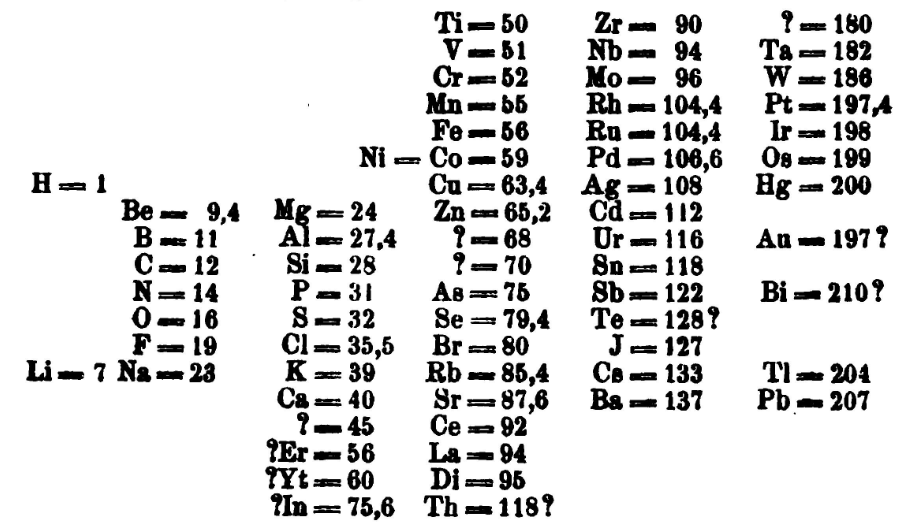
\includegraphics[width=0.7\textwidth]{figures/introduction/PeriodicTable.png}
    \caption{Dimitri Mendeleev's periodic table of elements from the late 1800s, taken from~\cite{MendeleevPaper}. The elements are grouped by similar chemical properties, and the gaps in the table are where Mendeleev predicted that new elements would be discovered.}
    \label{fig:periodic_table}
\end{figure}


Scientists' understanding of the building blocks of matter changed again around the turn of the 20th century, with physicists J.J. Thomson, Ernest Rutherford, and James Chadwick determining that the supposedly indivisible atom was composed of even smaller subatomic particles, eventually named electrons, protons, and neutrons~\cite{Electrons, Protons, Neutrons}. Thus the number of fundamental blocks of matter had decreased substantially from nearly 100 to just three. However, this number would need to be updated again only months later, as the fundamental anti-particle of the electron---known as the positron---was discovered in 1932 by Carl Anderson~\cite{Positron}. In the next two decades, the number of known fundamental particles would skyrocket. In 1947, the muon was discovered~\cite{Muon}, followed by the discovery of a laundry list of particles~\cite{Kaon,Lambda,Sigma} that participate in the same interaction that holds the positively charged protons together in the nucleus of an atom---the so-called \textbf{strong nuclear force}. These ``fundamental'' particles were collectively called \textbf{hadrons}, which were further separated into lighter and heavier categories, dubbed \textbf{mesons} and \textbf{baryons}, respectively~\cite{MesonBaryon}. By the late 1960s, the number of known hadrons had grown to well over 100~\cite{ParticleDiscoveries}, even more than the number of ``fundamental'' chemical elements that were known to exist in the 1800s.

In the same way that Mendeleev tried to group the elements by their similar chemical properties, physicists attempted to group the hadrons together based on their known subatomic properties. The first successful attempt at such a grouping was the \textbf{Eightfold Way}, which was independently proposed by Murray Gell-Mann and Yuval Ne'eman in 1961~\cite{GellMannEightfold, NeemanEightfold}. This grouping was found by examining the following properties of the hadrons:
%
\begin{enumerate}
    \item \textbf{Isotopic spin}: a quantum number introduced by Werner Heisenberg in 1932 to try to explain the apparent symmetries between the proton and neutron with respect to the strong nuclear force~\cite{IsotopicSpin} (i.e. although the proton and neutron have different electric charges, the strong interaction does not seem to distinguish between the two)
    \item \textbf{Strangeness}: another quantum number introduced by Gell-Mann and Nishijima in 1953 to explain why some hadrons decayed much more slowly than expected, and such particles appeared to be created in pairs~\cite{Strangeness}. In other words, the strong interaction responsible for the creation of these particles appeared to conserve this quantum number, but the weak interaction responsible for the slower decay of these particles did not. Strangeness\footnote{The ``strangeness'' being referred to in this section was introduced a few years before the very first quark model, but it now has the modern interpretation which is directly related to the number of strange and anti-strange quarks within a hadron.} will be discussed in more detail in Section~\ref{sec:flavor_conservation}.
\end{enumerate}
%
\begin{figure}[t!]
    \centering
    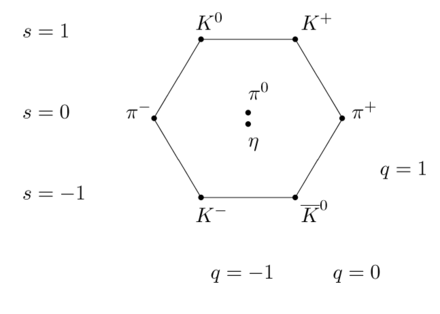
\includegraphics[width=0.49\textwidth]{figures/introduction/Meson_octet.png}
    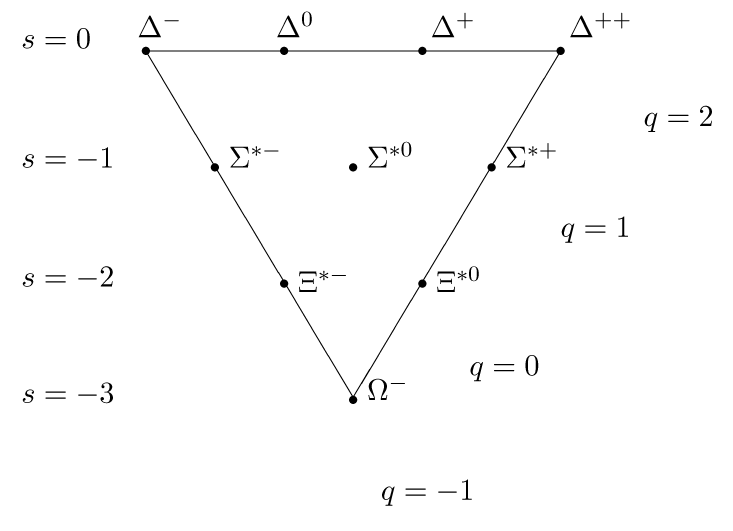
\includegraphics[width=0.49\textwidth]{figures/introduction/Baryon_decuplet.png}
    \caption{The ``Eightfold Way'' diagrams of the J = 1/2 mesons (left) and J = 3/2 baryons (right) plotted against strangeness and electric charge. Understanding the underlying symmetry group that gives rise to such patterns\protect\footnotemark \  ultimately led to the development of the quark model. While the original patterns were found using isotopic spin and hypercharge, it is trivial to convert between the two using the Gell-Mann-Nishijima formula~\cite{GellMannNishijima_1, GellMannNishijima_2}.}
    \label{fig:eightfold_way}
\end{figure}
\footnotetext{Namely SU(3), but this is a history lesson. Also the path from SU(3) to patterns of this type is long and arduous, involving a thorough understanding of representation theory.}
%

Plotting the baryons and mesons in a two-dimensional space based on these two properties revealed striking patterns, as shown in Figure~\ref{fig:eightfold_way}. Similar to Mendeleev, GellMann also left a blank space\footnote{The original paper on the Eightfold Way does not contain any of these diagrams, but there are discussions about the properties of particles that should exist if the theory were correct, but had not been observed~\cite{GellMannEightfold}.} where he believed a new particle--the $\Omega^{-}$--would be discovered.  The patterns in these diagrams hinted at an underlying symmetry governing the strong nuclear force, and ultimately led to the invention of the very first quark model by Gell-Mann and Zweig in 1964~\cite{QuarkModel}. This model proposed that all of the hadrons were actually composed of even smaller particles, which Gell-Mann dubbed ``quarks.'' The quark model was able to explain the patterns seen in Figure~\ref{fig:eightfold_way} by introducing three different types of fermionic quarks--up, down and strange--along with their corresponding anti-quarks. Baryons would then be composed of three such quarks, whereas mesons would be composed of quark and anti-quark pairs. If the quark model were correct, the number of fundamental building blocks of matter would again decrease from over 100 to just 14: electrons, muons, electron neutrinos, muon neutrinos, up quarks, down quarks, strange quarks, and all of their corresponding anti-particles.

Initially, many physicists believed that the quarks from this model were just a mathematical abstraction~\cite{QuarkAbstraction}. This possibility did not stop Sheldon Glashow and James Bjorken from extending the quark model less than a year after its inception by introducing a fourth quark: the charm~\cite{CharmQuark}. This new quark was primarily introduced to equalize the number of leptons (four at the time: electron, muon, and their respective neutrinos) with the number of quarks. The theory was mostly aesthetic~\cite{AestheticCharm} in that the charm quark was not explicity required by any known mechanisms. It was only after the Glashow-Iliopoulos-Maiani (GIM) mechanism was introduced in 1970~\cite{GIM} that the existence of the charm quark became necessary. This mechanism helped explain why neutral kaons decayed into two muons at a much lower rate than expected, but it required the existence of a quark with the same charge as the up quark but with a much larger mass.

 The notion that protons and neutrons were fundamental particles was also being challenged on the experimental side. The deep inelastic scattering experiments at the Stanford Linear Accelerator Center (SLAC) performed by Kendall, Friedman, and Taylor in 1968~\cite{Kendall, Friedman, Taylor} revealed unexpected\footnote{Depending on who you asked at the time, both the three and four quark models were not universally accepted.} behavior when probing the structure of the proton: it appeared to be composed of point-like particles. These experiments were performed by firing electrons at stationary protons and measuring the energy distributions of the scattered electrons at different scattering angles. An example of such a distribution for electrons with initial energies of 10 GeV scattered at 6 degrees can be seen in Figure~\ref{fig:dis}. The large spike on the left side of the distribution corresponds to the elastic scattering of the electron off the proton, which was well understood at the time~\cite{ElasticScattering}. The ``bumps'' observed at lower values of the scattered electron energy were also well understood~\cite{Resonances}, and they correspond to the ``shallow'' inelastic scattering of the electron off the proton, where the proton gets excited into a so-called \textit{resonance} state (like the $\Delta$ baryon). However, the ``background'' underneath the bumps and the apparent continuum of events at even lower values of the scattered electron energy corresponded to a host of unknown particles being produced. This host of particles appeared to grow with increasing scattering angle and decreasing scattered electron energy, which ultimately led to the conclusion that the proton was composed of point-like particles that were being ``knocked out'' of the proton by the incoming electron~\cite{Kendall, BjorkenScaling}.

\begin{figure}[ht]
    \centering
    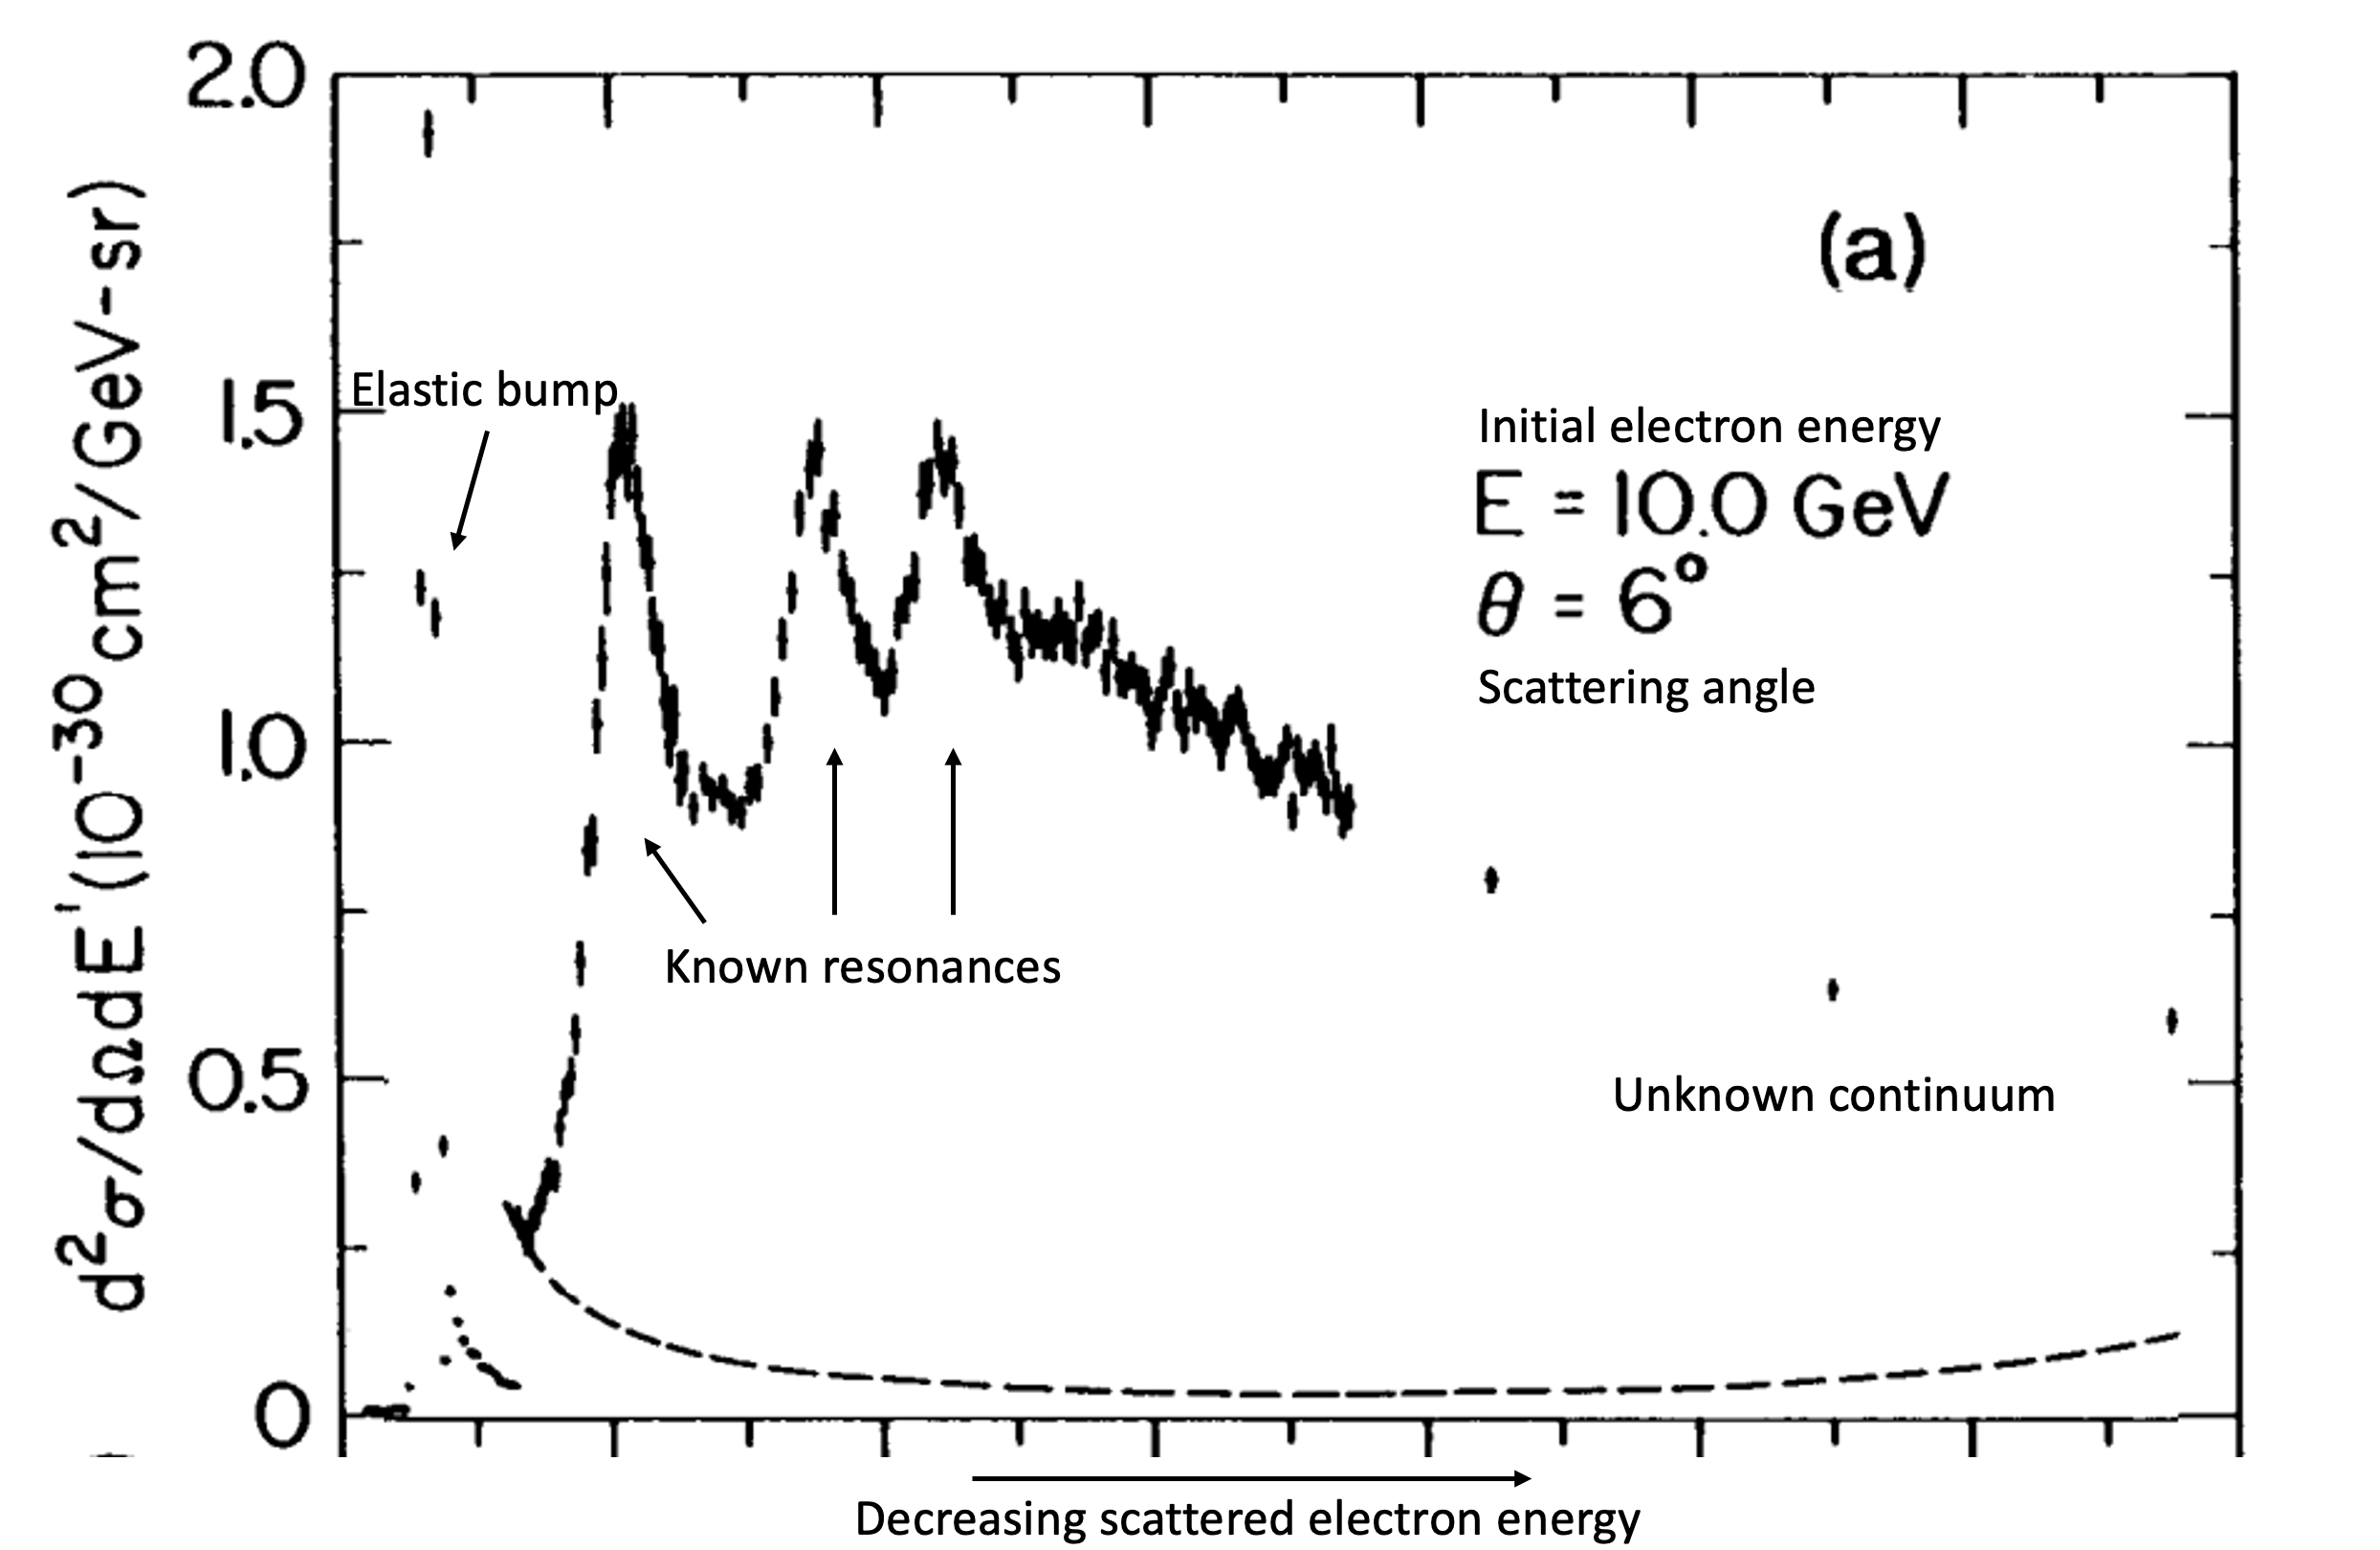
\includegraphics[width=0.7\textwidth]{figures/introduction/DeepInelasticScattering.png}
    \caption{The energy distribution of electrons scattered off of protons at an initial electron energy of 10 GeV and a scattering angle of 6 degrees. The large spike on the left side of the distribution corresponds to the elastic scattering of the electron off the proton, and the ``bumps'' correspond to the inelastic scattering of the electron off the proton. The ``background'' underneath the bumps and the apparent continuum of events at even lower values of the scattered electron energy correspond to a mess of unknown particles being produced. The behavior of this continuum with respect to the scattering angle and the scattered electron energy ultimately led to the conclusion that the proton was not fundamental.}
    \label{fig:dis}
\end{figure}

While many physicists were perfectly happy to interpret these point-like particles as the very same quarks from the aforementioned quark model(s), they received the much more noncommittal name \textbf{partons} after Richard Feynman's parton model of hadrons~\cite{Partons}. The association of these partons with quarks was not universally accepted\footnote{No acceptance of any model is a step function, but the discovery of J/$\psi$ seems to be a turning point in literature.} until the discovery of the J/$\psi$ meson in 1974~\cite{Jpsi}. In the meantime, the theoretical description of the strong nuclear force was closing in on its final form. The formulation of Quantum ChromoDynamics (QCD) in the early 1970s by Gell-Mann, Fritzsch, and Leutwyler~\cite{QCDFormulation} resolved many of the issues that were present in the initial quark models.\footnote{For example, the wavefunction of the $\Delta^{++}$ baryon under the first quark model was not antisymmetric, which is a requirement for fermions.} QCD introduced the concept of color charge, which all of the quarks would carry. The mediating bosons of the strong interaction--known as \textbf{gluons}--were also introduced, carrying color charge as well.

While QCD gave a solid mathematical description of the strong interaction, it wasn't until the discovery of \textbf{asymptotic freedom}~\cite{AssFreedom1, AssFreedom2} by Gross, Wilczek, and Politzer in 1973 that the theory became experimentally testable. Asymptotic freedom refers to the property that the strong interaction becomes weaker at higher energies, allowing for QCD calculations to be performed using perturbative techniques. This discovery allowed theorists to use QCD to make predicitions of the results of very high energy particle collision experiments. The first QCD prediction to be experimentally verified came from the Positron-Electron Tandem Ring Accelerator (PETRA) in 1979~\cite{PETRA}, which experimentally confirmed the existence of gluons~\cite{GluonConfirmation}. With experimental verification of QCD, it became clear that the association of partons with quarks was indeed incorrect: they are both quarks \textit{and} gluons.

In addition to the theory of QCD, the theory of electroweak interactions was also being developed during the 1960s by Glashow, Weinberg, and Salam~\cite{Electroweak1, Electroweak2}. With this new theory came the prediction of four\footnote{The Higgs mechanism (which predicts the existence of the Higgs boson) came before electroweak unification~\cite{HiggsPaper}, but it was a requirement for the theory.} new bosons: the Higgs boson, the charged W$^{\pm}$ bosons, and the neutral Z$^{0}$ boson. With the combined theories of the electroweak and strong interaction, the \textbf{Standard Model} of particle physics---which describes the now sixty-one\footnote{There are many ways to count fundamental particles, but this particular number is obtained by: 6 leptons ($\times 2$ for anti-leptons), 6 quarks ($\times 3$ for each color, $\times 2$ for anti-quarks), 1 gluon ($\times 8$ for color), 1 photon, the W and Z bosons, and the Higgs boson.} fundamental particles and how they interact---was complete. 

\clearpage

\section{The Standard Model}
\label{sec:standard_model}

The Standard Model of particle physics is a \textbf{quantum field theory} (QFT) that describes the interactions between all\footnote{Ignoring potential gravitons~\cite{Graviton} or dark matter candidates~\cite{DarkMatter1}} of the fundamental particles. QFTs describe the dynamics of a quantum system in terms of fields, which are functions of space and time. The fields are the fundamental objects of QFT, and their excitations correspond to the particles that are observed in nature. The Standard Model fields can be broken down into three sectors, which will be discussed in the following sections.

\subsection{The gauge sector}
\label{sec:gauge_fields}

The gauge sector of the Standard Model corresponds to the spin-one bosons that mediate the strong and electroweak interactions. In a general sense, this sector corresponds to the mediating particles for three of the four fundamental forces: the strong nuclear force, the weak nuclear force, and the electromagnetic force. The fourth fundamental force---gravity---is not included in the Standard Model, as it is not yet understood from a quantum perspective~\cite{QuantumGravity}.

The symmetry group of the gauge sector is given by
%
\begin{equation}
    \label{eq:gauge_symmetry}
    \text{SU(3)}_\text{c} \times \left[\text{SU(2)}_\text{L} \times \text{U(1)}_\text{Y}\right].
\end{equation}
%
SU(3)$_\text{c}$ is the symmetry group of the strong interaction, which is described by the QFT known as Quantum ChromoDynamics (QCD). The subscript c stands for ``color,'' indicating that the gauge fields in QCD (gluons) only couple to colored objects. QCD will be discussed in more detail in Section~\ref{sec:qcd}. The symmetry group of the electroweak interaction is SU(2)$_\text{L} \times$ U(1)$_\text{Y}$, where the subscript L stands for ``left-handed'' and the subscript Y stands for ``weak hypercharge.'' Again, these subscripts indicate the types of objects to which the corresponding gauge fields couple. For example, the gauge fields of SU(2)$_\text{L}$ only couple to left-handed objects, and the gauge fields of U(1)$_\text{Y}$ only couple to weakly hypercharged objects. Initially, there are four massless gauge fields in the electroweak theory.\footnote{Three corresponding to the generators of SU(2), one corresponding to the generator of U(1).} After the spontaneous symmetry breaking of the Higgs mechanism~\cite{HiggsPaper}, these fields mix to give rise to three massive gauge fields and one massless gauge field. The three massive gauge fields correspond to the familiar W$^{\pm}$ and Z$^{0}$ bosons, which are the mediating bosons of the weak interaction. The massless gauge field corresponds to the photon, which mediates the electromagnetic interaction.

\subsection{The scalar sector}
\label{sec:scalar_fields}

The scalar sector of the Standard Model is quite lonely, and only corresponds to one spin-zero field: the Higgs~\cite{HiggsPaper}. As mentioned in the previous section, the Higgs mechanism that corresponds to this field is responsible for the acquisition of mass by the W$^{\pm}$ and Z$^{0}$ bosons. The Higgs field also couples to all of the fermions in the Standard Model, but the mass acquisition procedure is \textit{slightly} different\footnote{It's still spontaneous symmetry breaking, but within the Yukawa part of the electroweak Lagrangian.} from the massive bosons. The associated Higgs boson was discovered by the A Toroidal LHC Apparatus (ATLAS) and Compact Muon Solenoid (CMS) collaborations in 2012~\cite{HiggsDiscovery1, HiggsDiscovery2}, and was the last major piece of the Standard Model to be experimentally verified.


\subsection{The fermionic sector}
\label{sec:fermion_fields}

The fermionic sector contains all of the spin one-half particles (quarks and leptons) in the Standard Model. It is often convenient to group these particles into three generations, where each generation is identical except for the masses of the particles. It is even \textit{more} convenient to group the fermions within each family into multiplets, where the members of the multiplet are related to each other by transformations within the gauge group of the Standard Model (Equation~\ref{eq:gauge_symmetry}). In other words, the fermions within a particular multiplet can only be transformed to fermions within the same multiplet. A table of the fermions in the Standard Model and their corresponding multiplets can be seen in Table~\ref{tab:fermions}. The indices $L$ and $R$ correspond to the chirality of the fields, and the indices $r$, $g$, and $b$  represent the color charge of the fields. The color charges are only non-zero for the quarks, making them the only fermions that couple to the gauge fields of the strong interaction (gluons).



\begin{table}
\caption{The fermions of the Standard Model for each generation and their corresponding multiplets. The Standard Model does not allow for fermions to leave their respective multiplets.}
\resizebox{\textwidth}{!}{%
\begin{tabular}{c|llllll}
\cline { 1 - 7 } Gen. & $\begin{array}{l} \text{Left-handed} \\ \text{quarks}\end{array}$ & $\begin{array}{l}\text { Right-handed } \\
\text { up quarks }\end{array}$ & $\begin{array}{l}\text { Right-handed } \\
\text { down quarks }\end{array}$ & $\begin{array}{l}\text { Left- } \\
\text { handed } \\
\text { leptons }\end{array}$ & $\begin{array}{l}\text { Right- } \\
\text { handed } \\
\text { leptons }\end{array}$ \\

\hline 

$1^{\text{st}}$ gen. & $\left(\begin{array}{lllll}u_L^r&u_L^g&u_L^b \\
d_L^r & d_L^g & d_L^b\end{array}\right)$ & $\left(\begin{array}{llll}u_R^r & u_R^g & u_R^b\end{array}\right)$ & $\left(\begin{array}{llll}d_R^r & d_R^g & d_R^b\end{array}\right)$ & $\left(\begin{array}{c}\nu_{e L} \\
e_L\end{array}\right)$ & $\left(e_R\right)$ \\

$2^{\text{nd}}$ gen. & $\left(\begin{array}{lllll}c_L^r & c_L^g & c_L^b \\
s_L^r & s_L^g & s_L^b\end{array}\right)$ & $\left(\begin{array}{llll}c_R^r & c_R^g & c_R^b\end{array}\right)$ & $\left(\begin{array}{llll}s_R^r & s_R^g & s_R^b\end{array}\right)$ & $\left(\begin{array}{c}\nu_{\mu_L} \\
\mu_L\end{array}\right)$ & $\left(\mu_R\right)$ \\
$3^{\text{rd}}$ gen. & $\left(\begin{array}{llll}t_L^r & t_L^g & t_L^b \\
b_L^r & b_L^g & b_L^b\end{array}\right)$ & $\left(\begin{array}{llll}t_R^r & t_R^g & t_R^b\end{array}\right)$ & $\left(\begin{array}{lll}b_R^r & b_R^g & b_R^b\end{array}\right)$ & $\left(\begin{array}{c}\nu_{\tau_L} \\
\tau_L\end{array}\right)$ & $\left(\tau_R\right)$

\end{tabular}}
\label{tab:fermions}
\end{table}

\clearpage

\section{Quantum chromodynamics}
\label{sec:qcd}

Quantum chromodynamics (QCD) is the component of the Standard Model that describes the strong interaction between quarks and gluons, the fundamental particles that make up most of the matter in the universe. In this theory, the fermionic quarks have ``color charge,'' which can either be red, green or blue for quarks, or anti-red, anti-green, or anti-blue for anti-quarks. The gluons, which are the mediating bosons of the strong interaction, also carry color charge, but in the form of a superposition of both color and anti-color. At everyday energies, these quarks and gluons are bound together in color-neutral states known as hadrons, like the protons and neutrons that compose the nuclei of atoms. These hadrons can be further grouped into two categories: \textit{mesons}, which are composed of a quark-anti-quark pair with opposite colors, and \textit{baryons}, which are composed of three quarks---one of each color.\footnote{Either (red, green, blue) or (anti-red, anti-green, anti-blue).} A diagram of a meson and baryon can be seen in Figure~\ref{fig:meson_baryon}.

\begin{figure}[h]
    \centering
    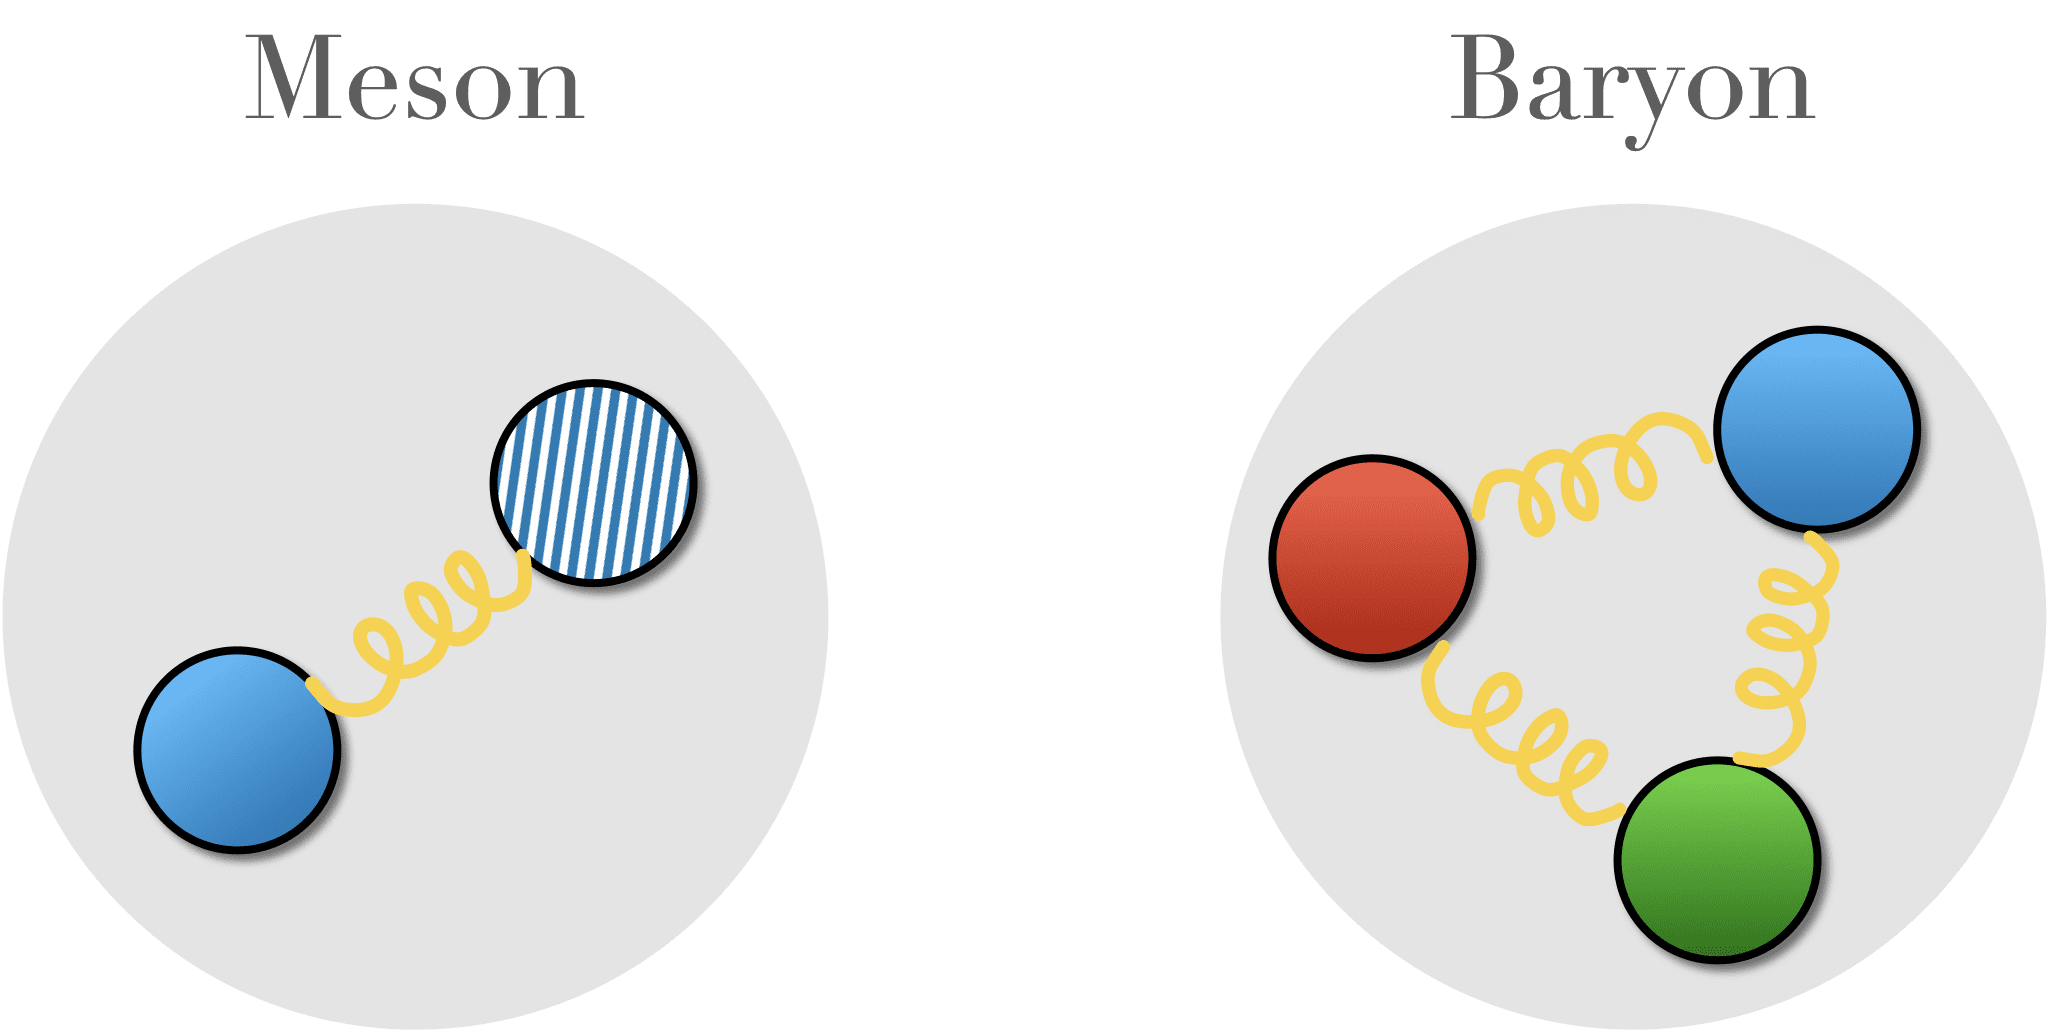
\includegraphics[width=0.7\textwidth]{figures/introduction/meson_baryon_figure.png}
    \caption{A diagram of a meson (left) and baryon (right). The meson is composed of a quark-anti-quark pair (blue-anti-blue), and the baryon is composed of three quarks (red, green, and blue).}
    \label{fig:meson_baryon}
\end{figure}


However, the full theory of QCD is more rich and complicated than this simple picture. As such, the remainder of this section will delve into the details of QCD, emphasizing the properties of the strong interaction that make it so challenging to study.

\subsection{The QCD Lagrangian}
\label{sec:qcd_lagrangian}

The dynamics of the Standard Model fields and how they interact are completely encoded within the Lagrangian of the theory, which can be used to calculate experimental observables like cross-sections and decay rates. However, the Lagrangian of the Standard Model is fairly long~\cite{StandardModelLength1}, and often not particularly insightful when trying to study a specific aspect of the theory. As such, when studying QCD, it is often useful to throw away the electroweak gauge fields, leptons, and scalars to look at only the QCD Lagrangian~\cite{QCDHistory},
%
\begin{align*}
    \label{eq:qcd_lagrangian}
    \mathcal{L}_{Q C D}= & -\frac{1}{4} F_{\mu \nu}^A F^{A \space \mu \nu}+i \bar{q} \gamma^\mu\left(\partial_\mu+i g_s \frac{1}{2} \lambda^A \mathcal{A}_\mu^A\right) q \\
    & -\bar{q}_{\mathrm{R}} \mathcal{M} q_{\mathrm{L}}-\bar{q}_{\mathrm{L}} \mathcal{M}^{\dagger} q_{\mathrm{R}}-\theta \omega,
\end{align*}
%
where all repeated indices are summed over.

The gluons are described by the vector gauge field $\mathcal{A}_\mu^A$, with index $A$ representing one of the eight color labels. These eight components belong to the color group SU$_\text{c}$(3), which is the gauge group of QCD. The corresponding coupling constant is $g_{s}$, and the field strength tensor $F_{\mu \nu}^A$ is given by
%
\begin{equation}
    \label{eq:field_strength_tensor}
    F_{\mu \nu}^A = \partial_\mu \mathcal{A}_\nu^A - \partial_\nu \mathcal{A}_\mu^A + g_s f^{ABC} \mathcal{A}_\mu^B \mathcal{A}_\nu^C,
\end{equation}
%
where $f^{ABC}$ are the structure constants~\cite{StructureConstants} of SU$_\text{c}$(3). Note that while this field strength tensor shares the same letters as the electromagnetic field strength tensor $F_{\mu \nu}$, the additional term $g_s f^{ABC} \mathcal{A}_\mu^B \mathcal{A}_\nu^C$ in Equation~\ref{eq:field_strength_tensor} separates QCD and QED in a very fundamental way: the gluons are allowed to self-interact. This self-interaction is a direct result of the non-vanishing structure constants of SU$_\text{c}$(3)\footnote{Structure constants of Abelian gauge groups like U(1) are trivially zero.}, and is responsible for the challenging nature of QCD calculations~\cite{QCDHistory}.

The quarks are represented by the field $q$, where the color, flavor and spin indices have been suppressed. In reality, the quark field $q$ has:
%
\begin{itemize}
    \item six flavor indices $\{u, d, s, c, b, t\}$,
    \item four spin indices $\{0, 1, 2, 3\}$, and
    \item three color indices $\{r, g, b\}$,
\end{itemize}
%
where all of these indices are being implicitly summed over in $\mathcal{L}_{QCD}$. Luckily, all of the matrices ($\mathcal{A}_\mu^A, \lambda^A, \mathcal{M}, \gamma^\mu$) act on separate sets of indices.\footnote{Really the components of the field corresponding to those indices.} For example, the $\gamma^\mu$s only operate on the spin indices, whereas the Gell-Mann matrices~\cite{GellMannEightfold} $\lambda^A$ operate on the color indices. These Gell-Mann matrices are the generators of SU$_\text{c}$(3), and they satisfy the commutation relation
%
\begin{equation}
    \label{eq:gell_mann_commutation}
    [\lambda^A, \lambda^B] = 2if^{ABC}\lambda^C.
\end{equation}
%
The chiral quark fields $q_\text{L}$ and $q_\text{R}$ are defined as $\frac{1}{2}(1 - \gamma_5)q$ and $\frac{1}{2}(1 + \gamma_5)q$, respectively. The mass matrix $\mathcal{M}$ operates on the flavor indices, and its form depends on the choice of basis for the quark fields~\cite{QCDHistory}. It is often convenient to choose a basis where the mass matrix is diagonal, which can be done by independent rotations of $q_\text{L}$ and $q_\text{R}$ in SU(6). Doing so gives the more familiar term
%
\begin{equation}
    -\bar{q}_{\mathrm{R}} \mathcal{M} q_{\mathrm{L}}-\bar{q}_{\mathrm{L}} \mathcal{M}^{\dagger} q_{\mathrm{R}} = -\sum_{f = 1}^{6}\bar{q}_f m_f q_f,
    \label{eq:mass_matrix}
\end{equation}
where $m_f$ is the mass of the quark with flavor $f$, and $q_f$ is the flavor component of the quark field. Note that this term completely violates the SU(2)$\times$U(1) electroweak symmetry, indicating that the given $\mathcal{L}_{QCD}$ is determined \textit{after} the spontaneous symmetry breaking described in the previous section. 

These quark masses are also subject to \textbf{renormalization}~\cite{MassRenorm}, which is the process of removing the infinities in QFT calculations by redefining the parameters of the theory. In QCD, renormalization results in the running of the quark masses with respect to the energy scale $\mu$ of the interaction.\footnote{They also depend on the \textit{choice} of renormalization scheme, with the most commonly implemented one being minimal subtraction or MS~\cite{MSScheme}.} More simply, the quark masses are inversely dependent on this energy scale: at large $\mu$, the quark masses are small, and at small $\mu$, the quark masses are large. At the energy scale $\mu \approx 2$ GeV (close to the mass of the proton), the masses of the up, down, and strange quarks---collectively referred to as the light-flavor quarks---are approximately 2.2 MeV/$c^2$, 4.7 MeV/$c^2$, and 96 MeV/$c^2$, respectively~\cite{PDG}. The heavy-flavor charm, bottom, and top quarks have masses of approximately 1.28 \GeVmass, 4.18 \GeVmass, and 173 \GeVmass, respectively.\footnote{At the energy scale governed by their respective masses (i.e. $\mu = m_{Q}$).~\cite{PDG}} 

The final term, known as the $\theta$-term~\cite{ThetaTerm}, is something of a mystery. It is a scalar term that violates CP symmetry~\cite{CPSymmetry}, and is often set to zero as there is no experimental evidence for its existence. However, it is not clear why this term is zero, as there is no symmetry that explicitly forbids it. This is known as the \textbf{strong CP problem}, and is one of the biggest open questions in particle physics~\cite{StrongCPProblem}. 


\subsubsection{Brief aside: Why eight gluons?}
\label{sec:why_eight_gluons}

The gluon field $\mathcal{A}^A$ transforms under the adjoint respresentation of SU(3), which is a representation of SU(3) on the vector space of its Lie algebra $\mathfrak{su}(3)$. As $\mathfrak{su}(3)$ has eight basis elements (for instance, the Gell-Mann matrices $\lambda^A$ from above), the adjoint representation of SU(3) is eight-dimensional. Thus the gluon field has eight independent components, or, equivalently, there are eight gluons. In principle, QCD could have been built on top of a U(3) gauge group, which would give rise to nine gluons (as the dimension of U(n) is $n^2$). However, the singlet state in U(3) would be required to be non-interacting; if it were, color neutral baryons would interact with each other via the strong interaction at a much longer range~\cite{SingletGluons}. Such interactions have not been observed~\cite{SingletGluons2}. As there is no physical difference between U(3) with a non-interacting singlet and SU(3), the simpler gauge group was chosen. 


\subsection{Properties of QCD}
\label{sec:qcd_properties}

\subsubsection{Confinement}
\label{sec:qcd_confinement}

One of the unique properties of QCD is the phenomenon of \textbf{confinement}, which is the observation that quarks and gluons are never seen in isolation. Instead, they are \textit{confined} inside of the color neutral bound states known as hadrons. This property is mostly understood in terms of the coupling constant $g_{s}$. The renormalization~\cite{QCDRenorm} of QCD gives rise to a $g_{s}$ that varies with energy scale or distance. As the distance between two quarks increases, so too does $g_{s}$. At some point, the coupling becomes so strong that the energy required to separate the quarks is enough to create a quark-anti-quark pair from the vacuum. Thus any attempts to separate a quark from a hadron will always result in the creation of a new hadron, making it impossible to observe single quarks in isolation. 

The large coupling constant in this low energy regime makes it impossible to describe this phenomenon using perturbative techniques, so the exact mechanism of confinement is still not fully understood. However, it is often described using the phenomenological Lund string model~\cite{LundString}. In this model, the field lines of two quarks are pulled together due to the self-interaction of the gluons. This creates a string-like structure between the two quarks, with a potential given by 
%
\begin{equation}
    \label{eq:lund_potential}
    V(r) \approx -\frac{4}{3}\frac{\alpha_s}{r} + \kappa r,
\end{equation}
%
where $r$ is the distance between the two quarks, $\alpha_s = \frac{g_s^2}{4\pi}$ and $\kappa$ is the string tension. This can be contrasted with the potential between two electrically charged particles, where the field lines are not pulled together and become less dense as the distance between the two particles increases. As such, the potential decreases with increasing distance, opposite to that of the Lund model. A schematic of these differences can be seen in Figure~\ref{fig:field_line_differences}. Pulling the quarks apart eventually ``breaks'' the Lund string, forming two separate quark-anti-quark pairs, as shown in the bottom right of the figure.

\begin{figure}[ht]
    \centering
    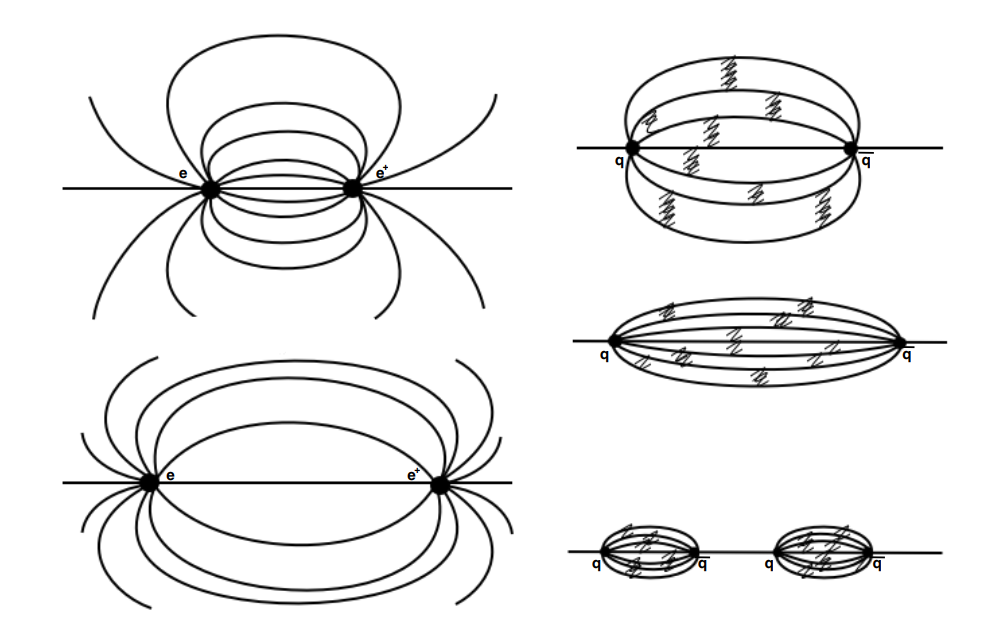
\includegraphics[width=0.7\textwidth]{figures/introduction/electric_color_fields.png}
    \caption{A schematic of the field lines between two electrically charged particles (left) and two quarks (right). The field lines between the quarks are pulled together due to the self-interaction of the gluons, whereas the electic field lines are not.}
    \label{fig:field_line_differences}
\end{figure}

\subsubsection{Asymptotic freedom}
\label{sec:qcd_asymptotic_freedom}

Just as the coupling constant becomes large at low energies and large distances, it also becomes small at high energies and small distances. This property is known as \textbf{asymptotic freedom}: at high enough energies, the quarks and gluons can be thought of as ``free,'' and their interactions can be modeled using perturbative QCD (pQCD). As discussed in Section~\ref{sec:fundamental}, the discovery of asymptotic freedom in QCD was what allowed for the accurate predictions of the results of high energy particle collision experiments like SLAC~\cite{SLAC} and PETRA~\cite{PETRA}. The results of such experiments have also been used to calculate the value of the coupling constant itself at different energy scales, as shown in Figure~\ref{fig:asymptotic_freedom}. The value of $\alpha_s$ at the Z$^0$ mass is also given in the figure, which is the most accurate measurement of $\alpha_s$ to date~\cite{PDG}. 

\begin{figure}
    \centering
    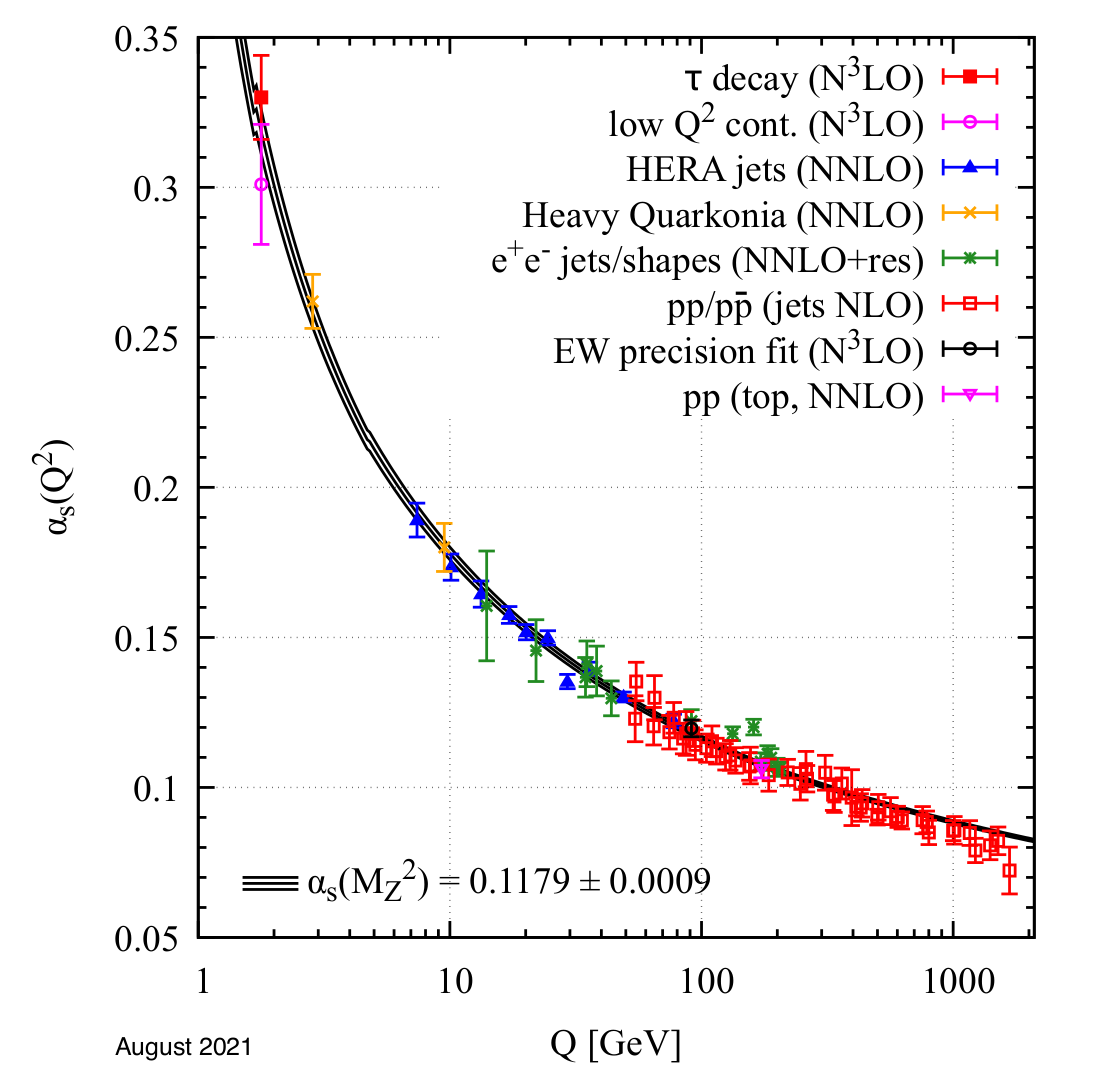
\includegraphics[width=0.7\textwidth]{figures/introduction/running_coupling.png}
    \caption{The value of the strong coupling constant $\alpha_s$ as a function of momentum transfer $Q$, which represents the energy scale of the interaction.}
    \label{fig:asymptotic_freedom}
\end{figure}

\subsubsection{Chiral symmetry breaking}
\label{sec:chiral_symmetry_breaking}

The mass term in the QCD Lagrangian,
\begin{equation}
    -\bar{q}_{\mathrm{R}} \mathcal{M} q_{\mathrm{L}}-\bar{q}_{\mathrm{L}} \mathcal{M}^{\dagger} q_{\mathrm{R}},
\end{equation}
explicitly breaks \textbf{chiral symmetry}: independent rotations of $q_\text{L}$ and $q_\text{R}$ in flavor-space (i.e. SU(6)) do not leave the Lagrangian invariant. The breaking of chiral symmetry due to the non-zero quark masses is referred to as \textbf{explicit} chiral symmetry breaking.

However, even in the limit of massless quarks, chiral symmetry is broken by the QCD vacuum. This is known as \textbf{spontaneous} chiral symmetry breaking, which is due to the non-zero vacuum expectation value of the quark condensate~\cite{QuarkCondensate}
%
\begin{equation}
    \label{eq:quark_condensate}
    \langle \bar{q}q \rangle = \langle \bar{q}_\text{L}q_\text{R} + \bar{q}_\text{R}q_\text{L} \rangle \neq 0.
\end{equation}
%
This non-zero value is a direct result of the confinement of QCD~\cite{TongGaugeTheory} (Section~\ref{sec:qcd_confinement}), and implies that the ground state of the theory is filled with quark-anti-quark pairs. The spontaneous breaking of chiral symmetry in QCD gives rise to eight massless Nambu-Goldstone bosons~\cite{NambuGoldstone}, which are the pseudoscalar mesons $\pi^{\pm, 0}$, $K^{\pm, 0}$, $\eta$, and $\eta'$. These mesons then acquire a small mass due to the aforementioned explicit chiral symmetry breaking from the quark masses. 

\subsubsection{Jets}
\label{sec:jets}

During high energy particle collisions (between two protons, for example), the constituent partons of the protons will sometimes scatter off each other in a way that converts most of their initial longitudinal momentum (along the collision axis) into transverse momentum (in the plane perpendicular to the collision axis). Such a scattering is often referred to as a \textbf{hard scattering}. Because the momentum transfer is large, the cross-section of the parton-parton scattering is calculable using pQCD. Furthermore, branching processes of the high momentum partons---like gluon radiation---can also be calculated perturbatively. Eventually, however, the partons will lose enough energy such that their behavior can no longer be described using perturbative techniques.

Luckily, the aforementioned Lund model is well-equipped to deal with lower energy partons. Under the Lund model, as these colored partons move away from each other, the force between them increases until there is enough energy to produce a quark-anti-quark pair (as discussed in Section~\ref{sec:qcd_confinement}). This process---known as string fragmentation---continues until the partons are no longer energetic enough to move away from each other, at which point they hadronize into a large number of color neutral bound states. These particles are roughly collimated in the direction(s) of the initial hard scattering, forming sprays of hadrons known as \textbf{jets}. A diagram depicting the formation of a jet from an initial hard scattering of partons can be seen in Figure~\ref{fig:jet_diagram}. 

\begin{figure}[ht]
    \centering
    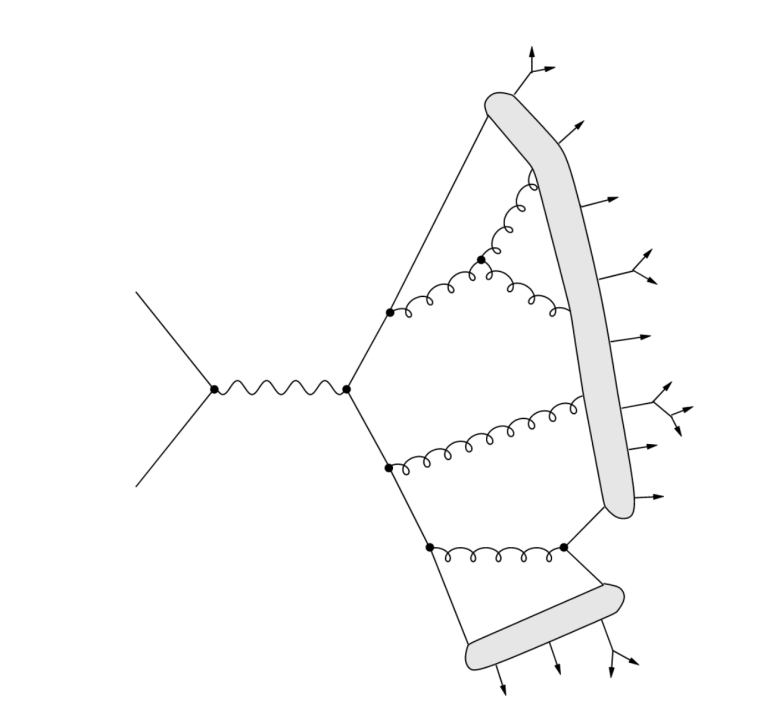
\includegraphics[width=0.7\textwidth]{figures/introduction/jet_string.png}
    \caption{A diagram depicting the formation of a jet within the Lund model from an initial hard scattering of partons, adapted from~\cite{JetStringDiagram}. The vertices represent perturbative QCD processes, the shaded regions represent string fragmentation/hadronization, and the outgoing arrows represent the resulting hadrons (which may decay further).}
    \label{fig:jet_diagram}
\end{figure}

\subsubsection{Flavor conservation}
\label{sec:flavor_conservation}

One interesting feature of the interactions in QCD is that all \textbf{flavor} quantum numbers are conserved. Specifically, the number of quarks minus the number of anti-quarks of each flavor is a conserved quantity in every strong interaction.\footnote{Conservation of the ``historical'' flavor quantum number \textit{isospin} (from Section~\ref{sec:fundamental}), which is $+\frac{1}{2}$ for up quarks and $-\frac{1}{2}$ for down quarks, is equivalent to the conservation of $n_{u,d} - n_{\bar{u}, \bar{d}}$ when baryon number is considered. Baryon number is an absolutely conserved quantum number in the Standard Model~\cite{PDG}, and (anti-)quarks have baryon number (-)$\frac{1}{3}$.'} In this thesis, the most important flavor quantum number is \textbf{strangeness}, which is defined as
%
\begin{equation}
    \label{eq:strangeness}
    S = - (n_s - n_{\bar{s}}),
\end{equation}
where $n_s$ is the number of strange quarks and $n_{\bar{s}}$ is the number of strange anti-quarks. The ``minus'' sign in front of the expression indicates that the strangeness of a strange quark is negative ($-1$), and the strangeness of a strange anti-quark is positive ($+1$). This convention is chosen\footnote{Really this is a historical convention that stems from the fact that ``strangeness'' was introduced as a concept before the existence of any quark models, as mentioned in Section~\ref{sec:fundamental}.} to make the signs of these ``flavor charges'' consistent with the signs of the electric charges of these quarks, which are $-\frac{1}{3}$ for the strange quark and $+\frac{1}{3}$ for the strange anti-quark. 

Strangeness conservation has an interesting consequence for particle collisions between atomic nuclei: as the total strangeness of these nuclei (protons and neutrons) is zero, the number of strange and anti-strange quarks produced from the strong interaction during these collisions must be equal. In other words, the production of strange quarks in these collisions must come in the form of strange quark-anti-quark ($s\bar{s}$) pairs.

\clearpage

\section{The Quark-Gluon Plasma}
\label{sec:qgp_theory}

One of the consequences of the asymptotic freedom of QCD is the possibility of a new state of matter at extreme temperatures and densities: the \textbf{quark-gluon plasma} (QGP) ~\cite{QGP1, QGP2}. In this plasma, the quarks and gluons are not confined inside hadrons, and instead behave as quasi-free particles. This is analogous to an electromagnetic plasma, where electrons and protons are dissociated from their atoms. A phase diagram of QCD matter showing the transition between hadronic matter and the QGP can be seen in Figure~\ref{fig:qgp_phase_diagram}. This diagram has two axes: temperature and baryon density. Increasing \textit{either} of these quantities beyond a certain threshold will cause a phase transition from normal hadronic matter to the QGP. Similarities can be drawn between this phase diagram and that of a snowball: heating \textit{{or}} squeezing a snowball will cause it to melt into a liquid.\footnote{Be careful: if you continue to heat up the snowball enough, or squeeze hard enough, it will undergo another phase transition into the QGP.}  

\begin{figure}[h]
    \centering
    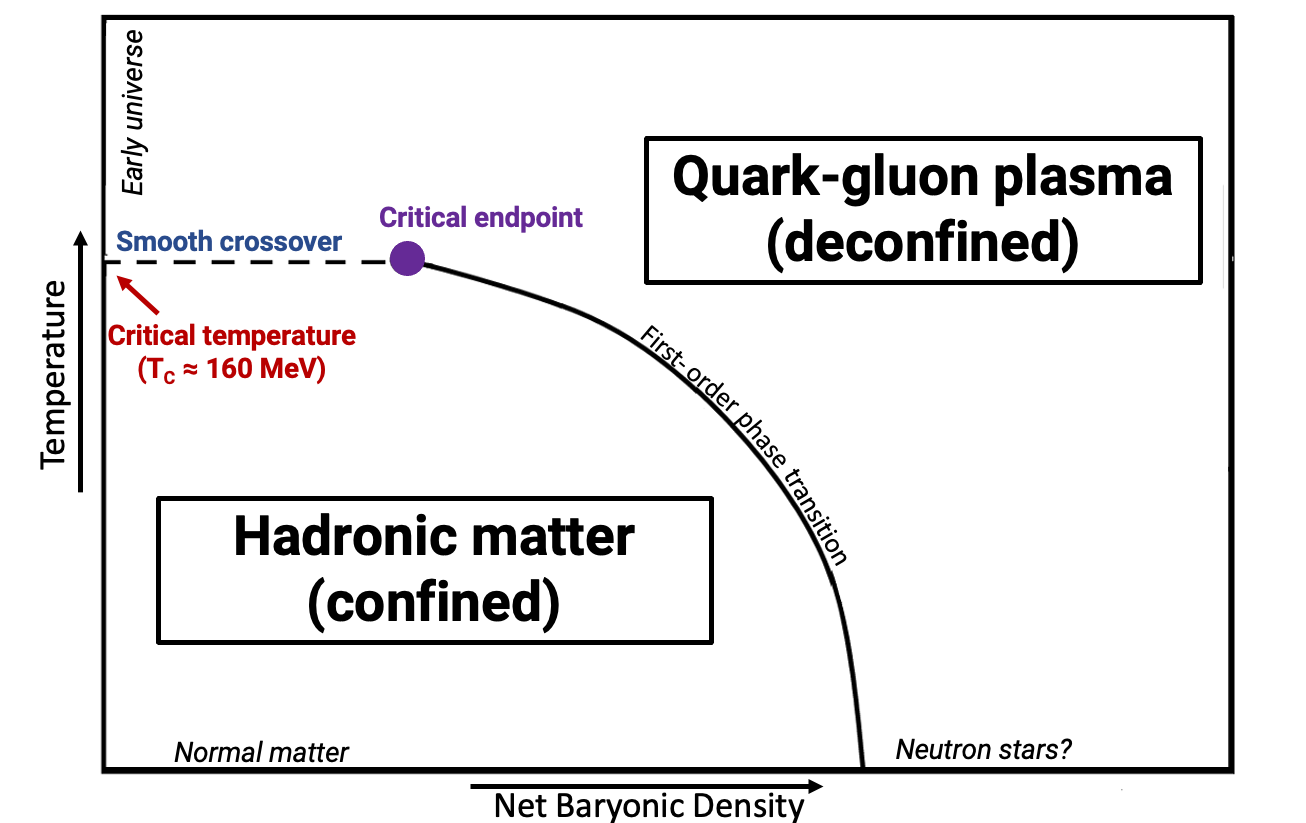
\includegraphics[width=0.8\textwidth]{figures/introduction/qgp_phase_diagram.png}
    \caption{A phase diagram of QCD matter, where the axes are temperature and baryon density. The dashed line represents the region in which lQCD predicts a smooth crossover between hadronic matter and the QGP, with a critical temperature $T_{C} \approx 160$ MeV. The critical endpoint is the point at which the smooth crossover ceases, above which the phase transition becomes first-order.}
    \label{fig:qgp_phase_diagram}
\end{figure}

\clearpage

Numerical simulations of QCD on a lattice~\cite{LatticeQCD1, LatticeQCD2} (known as lattice QCD or lQCD) have shown that at zero baryon density, the transition from hadronic matter to the QGP occurs as a smooth crossover~\cite{Crossover1, Crossover2} with a critical temperature $T_C \approx 160$ MeV or $10^{12}$ K, which is over 10,000 times hotter than the center of the sun. LQCD has also been used to predict the existence of a critical endpoint in the QGP phase diagram at a non-zero baryon density~\cite{CriticalEndpoint}, beyond which the transition from hadronic matter to the QGP is no longer a smooth crossover, but a first-order phase transition. However, due to the complex action problem~\cite{ComplexAction} (also known more generally as the ``sign problem''), lQCD simulations at non-zero baryon densities are extremely difficult.\footnote{Though there are plenty of techniques to extend the lQCD results~\cite{TaylorSeries, ComplexDensity}, they are only applicable at small baryon densities.} Thus the exact location of this critical endpoint is still unknown, and is the subject of much experimental and theoretical research~\cite{QGP3}.

\begin{figure}[t!]
    \centering
    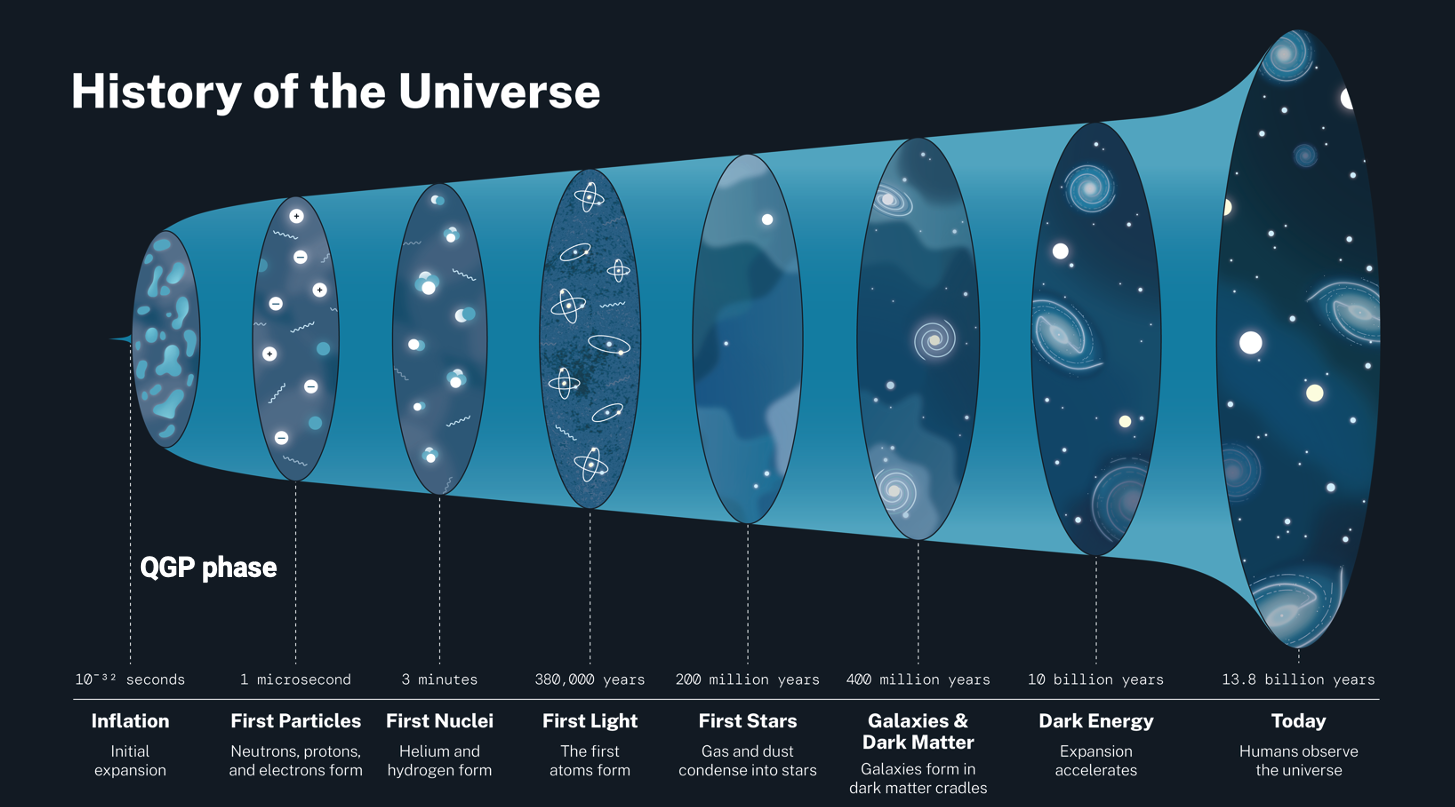
\includegraphics[width=0.8\textwidth]{figures/introduction/qgp_history.png}
    \caption{A schematic of the evolution of the universe. The QGP phase of the universe on this diagram lies roughly between 10$^{-10}$ and 10$^{-6}$ seconds after the Big Bang. Credit: NASA}
    \label{fig:qgp_universe}
\end{figure}

As the temperatures at the early stages of the universe were much larger than 160 MeV, it is thought that the universe was filled with a QGP in the first few microseconds after the Big Bang~\cite{QGP3}. Thus studying the QGP is of interest to cosmologists, as it can give insight to the early universe and its expansion, which is schematically represented in Figure~\ref{fig:qgp_universe}. It is also postulated that QGP formation occurs in the cores of neutron stars~\cite{QGPNeutron}, giving another avenue of interest for astrophysicists. Furthermore, studying the QGP and its properties can help illuminate the dark, confounding corners of QCD that are not yet understood from first principles---like confinement---making it an exciting area of research for particle physicists. The remainder of this section will discuss the theoretical characteristics of this interesting plasma.


\subsection{Properties of the QGP}
\label{sec:qgp_properties}

\subsubsection{Deconfinement}

The most defining characteristic of the QGP is that the quarks and gluons within the plasma are not confined inside hadrons, and instead interact as quasi-free particles. As mentioned in Section~\ref{sec:qcd_asymptotic_freedom}, the coupling constant $g_s$ becomes smaller with increasing energies. At high enough energies, the coupling constant becomes small enough that the quarks and gluons become \textit{deconfined}. In lQCD, the order parameter for deconfinement is the Polyakov loop expectation value~\cite{PolyakovLoop} $\langle L \rangle$, which is zero in the confined phase and greater than zero in the deconfined phase. This transition (from $\langle L \rangle = 0$ to $\langle L \rangle > 0$) is used to define the transition from hadronic matter to the QGP. 


\subsubsection{Chiral symmetry restoration}

As mentioned in Section~\ref{sec:chiral_symmetry_breaking}, the QCD vacuum has a non-zero quark condensate $\langle q\bar{q} \rangle$ which spontaneously breaks chiral symmetry. However, this non-zero condensate is the direct result of the confinement of QCD~\cite{TongGaugeTheory}. Thus, within the QGP---where the quarks and gluons are no longer confined---the quark condensate should vanish. As such, another defining characteristic of the QGP is the restoration of the spontaneously broken chiral symmetry of QCD, often referred to as \textbf{chiral symmetry restoration}. The transition from $\langle q\bar{q} \rangle > 0$ (broken chiral symmetry) to $\langle q\bar{q} \rangle = 0$ (restored chiral symmetry) is \textit{also} used to define the QGP phase transition. 

An lQCD diagram of the deconfinement order parameter $\langle L \rangle$ and chiral symmetry order parameter $\langle q\bar{q} \rangle$ (along with their corresponding susceptibilities) as a function of the coupling $\beta = 6/g_s^2$ can be seen in Figure~\ref{fig:order_parameters}. Note that the susceptibilities are maximal at the same coupling value (corresponding to a critical temperature of around 170 MeV), indicating that both deconfinement and chiral symmetry restoration correspond to the same phase transition. Namely, the transition from hadronic matter to the QGP.

\begin{figure}
    \centering
    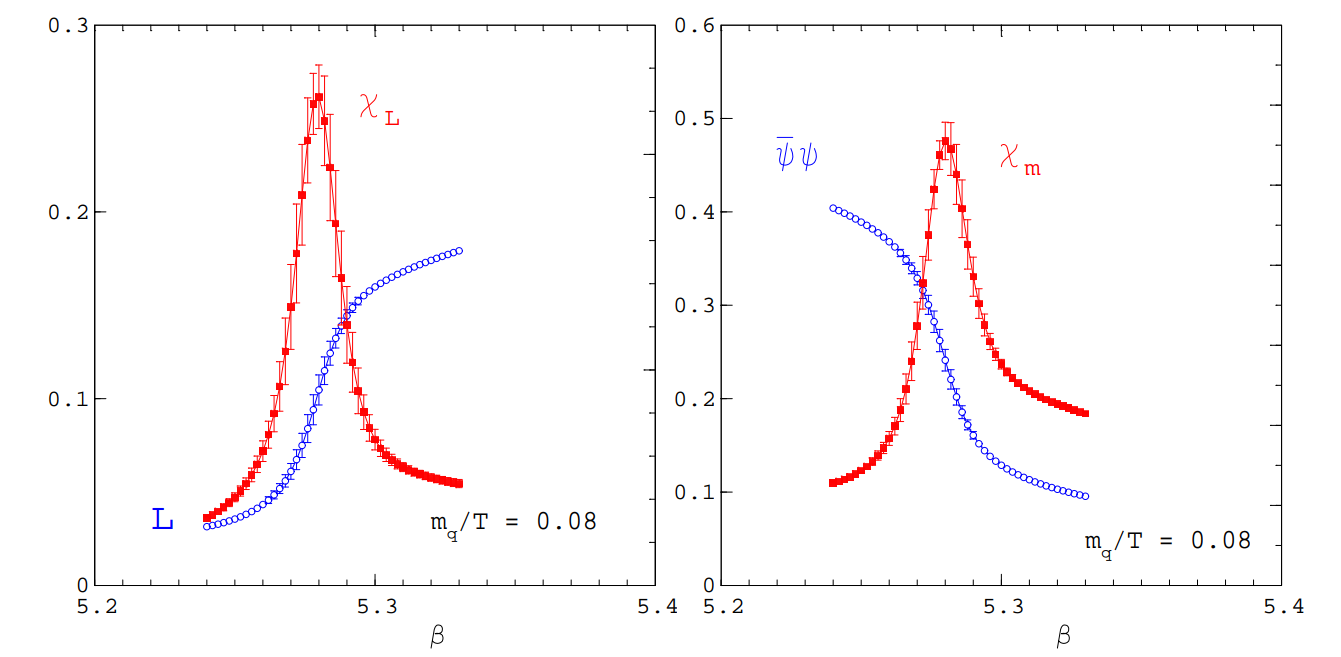
\includegraphics[width=0.9\textwidth]{figures/introduction/phase_transition.png}
    \caption{The deconfinement order parameter $\langle L \rangle$ and chiral symmetry order parameter $\langle q\bar{q} \rangle$ (along with their corresponding susceptibilities) as a function of the coupling $\beta = 6/g_s^2$ using 2-flavor lQCD, taken from~\cite{FrithofLattice}. The critical temperatures (indicated by the maxima of the susceptibilities) occur at roughly $\beta = 5.28$, corresponding to a temperature of around 170 MeV.}
    \label{fig:order_parameters}
\end{figure}

\subsubsection{Hydrodynamic behavior}
\label{sec:qgp_fluid}

The QGP is a strongly interacting plasma. As such, it is expected to exhibit fluid-like behavior at a macroscopic level. Unfortunately, the calculation of QGP transport coefficients from first principles using QCD is very difficult~\cite{FlowViscPaper}. Using perturbative techniques to calculate the shear and bulk viscosities of the QGP results in values that are an order of magnitude larger than those extracted from experimental data~\cite{Visc1}. The extraction of these transport coefficients using lQCD is also challenging, as the aforementioned complex action problem makes it nearly impossible to simulate the QGP at non-zero baryon density. The most promising approach to calculating these transport coefficients is through the use of the AdS/CFT correspondence~\cite{AdSCFT}, which is a duality between a strongly coupled gauge theory (like QCD) and a weakly interacting gravitational theory (like string theory~\cite{StringTheory}). This approach has been used to approximate the lower bound of the shear viscosity of a strongly-coupled medium~\cite{QGPViscADS}, 
\begin{equation}
\eta/s \approx 1/4\pi,
\end{equation}
which is often described as the shear viscosity of a ``perfect fluid.'' Experimental evidence suggests that the QGP has a shear viscosity that is very close to this lower bound~\cite{QGPViscExp}, indicating that it is a nearly perfect fluid.


\subsubsection{Radiative energy loss}
\label{sec:qgp_energy_loss}

Partons traveling through the QGP lose energy through both collisional and radiative processes, as shown in Figure~\ref{fig:energy_loss_qgp}. The collisional energy loss is due to the elastic scatterings between the parton and the constituents of the QGP. For a parton with energy $E$ much greater than its mass and the temperature of the QGP, the collisional energy loss is given by~\cite{GluonRadiation}
%
\begin{equation}
    \label{eq:collisional_energy_loss}
    \Delta E_\text{coll} \sim \alpha_s^2 T^2 L,
\end{equation}
%
where $T$ is the temperature of the QGP and $L$ is the length of travel through the medium (which is assumed to be larger than the critical length $L_{cr} \sim \frac{1}{\alpha_s T}\sqrt{\frac{E}{T}}$). 

\begin{figure}[h]
    \centering
    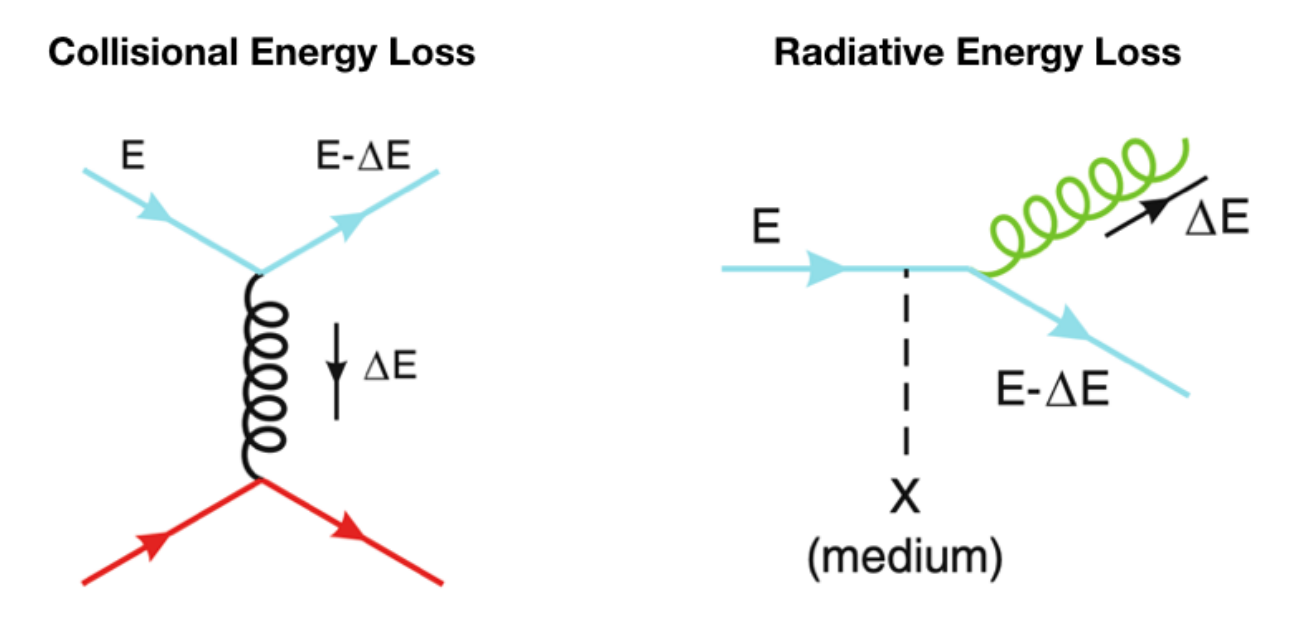
\includegraphics[width=0.8\textwidth]{figures/introduction/energy_loss.png}
    \caption{A diagram depicting the collisional (left) and radiative energy loss (right) processes of a parton traveling through the QGP. Radiative energy loss is the dominant energy loss mechanism for all energetic partons in the QGP.}
    \label{fig:energy_loss_qgp}
\end{figure}

The radiative energy loss is due to gluon radiation, induced by the presence of the medium.\footnote{Similar to bremsstrahlung, where electrically charged particles radiate photons in the presence of other charged particles.} Again, for a parton with $E >> M, T$, the radiative energy loss is given by
%
\begin{equation}
    \label{eq:radiative_energy_loss}
    \Delta E_\text{rad} \sim \alpha_s^2 \sqrt{E T^3} L,
\end{equation}
%
where $E$ is the energy of the parton. As the radiative energy loss is proportional to $\sqrt{E}$, it is the dominant energy loss mechanism for light, energetic partons (i.e. $u$, $d$, and $s$ quarks as well as gluons). However, gluons are expected to lose more energy than the light quarks due to their larger color charge. 

The heavier quarks ($b$, $c$) are expected to lose less energy through radiative processes than the lighter quarks and gluons due to the \textit{dead cone effect}, whereby the gluon radiation is suppressed in the forward direction due to the larger masses of the heavy quarks~\cite{DeadCone}. Even still, the radiative energy loss of heavy quarks is larger than their collisional energy loss, making radiative energy loss the dominant energy loss mechanism for all energetic partons in the QGP.



\subsection{Enhanced $s$-quark production}
\label{sec:qgp_strangeness}

In the context of the research presented in this thesis, the most important characteristic of the QGP is the increase in the production of strange quarks when compared to strange quark production within a hadronic gas~\cite{Strangeness}. Predicted in 1981 by physicists Johann Rafelski and Rolf Hagedorn, this \textit{enhancement} in the production of strange quarks in the QGP is often referred to as \textbf{strangeness enhancement}. As mentioned in Section~\ref{sec:flavor_conservation}, strangeness is conserved during strong interactions. As such, the production of $s\bar{s}$ pairs can only come from four Feynman diagrams (to lowest order in pQCD), shown in Figure~\ref{fig:ssbar_production}. A key insight made by Rafelski and Hagedorn is that in the QGP, the higher temperatures allow for the thermal production of $s\bar{s}$ pairs through gluon fusion ($gg \rightarrow s\bar{s}$ or diagrams (a) (b) and (c) in Figure~\ref{fig:ssbar_production}). This gluon fusion occurs much faster than the quark-based production ($q\bar{q} \rightarrow s\bar{s}$ or diagram (d) in Figure~\ref{fig:ssbar_production}), and allows for the full chemical equilibration of strangeness in the QGP in a very short time frame. For a QGP at 160 MeV, this equilibration can occur in less than $10^{-22}$ seconds, as shown in Figure~\ref{fig:qgp_equil}. Also shown in the figure is the strangeness equilibration time for a hadronic gas at the same temperature, which is nearly 100 times slower.


\begin{figure}[ht]
    \centering
    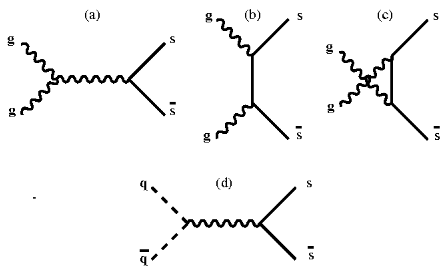
\includegraphics[width=0.7\textwidth]{figures/introduction/ssbar_production.png}
    \caption{The four leading-order Feynman diagrams responsible for the production of $s\bar{s}$ pairs in the QGP, adapted from~\cite{Strangeness}. Diagrams (a), (b) and (c) are the gluon fusion processes, while diagram (d) is the quark-based process.}
    \label{fig:ssbar_production}
\end{figure}

\begin{figure}
    \centering
    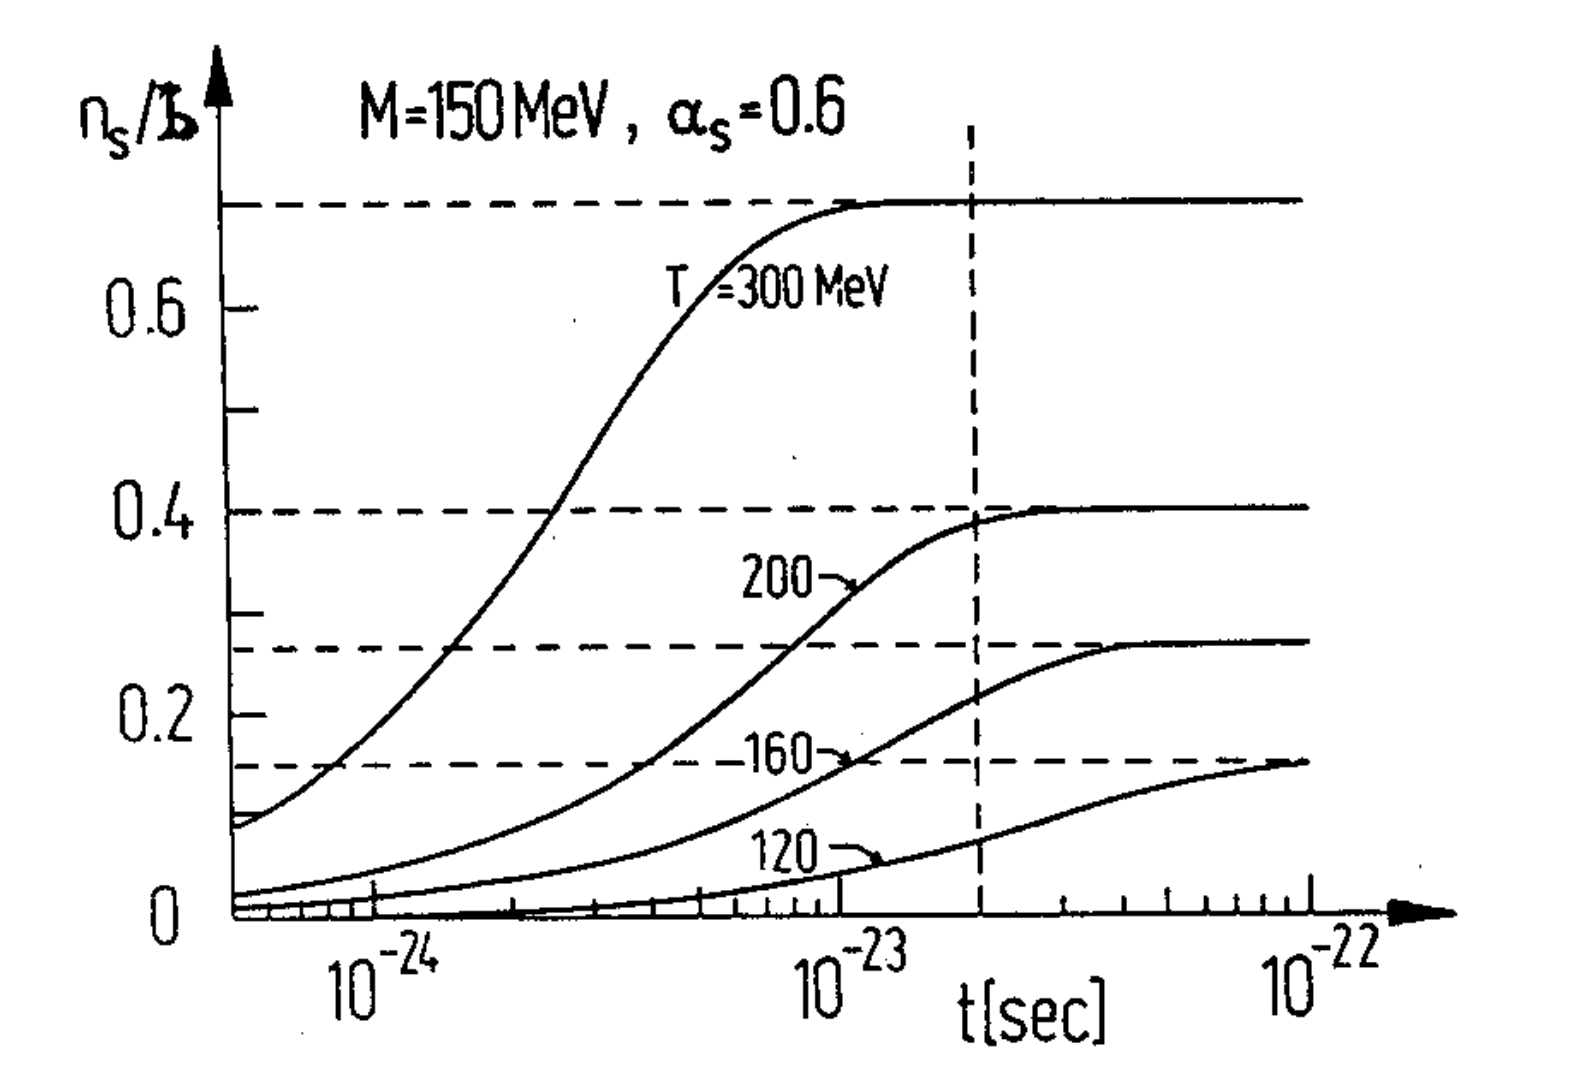
\includegraphics[width=0.6\textwidth]{figures/introduction/plasma_equil.png}
    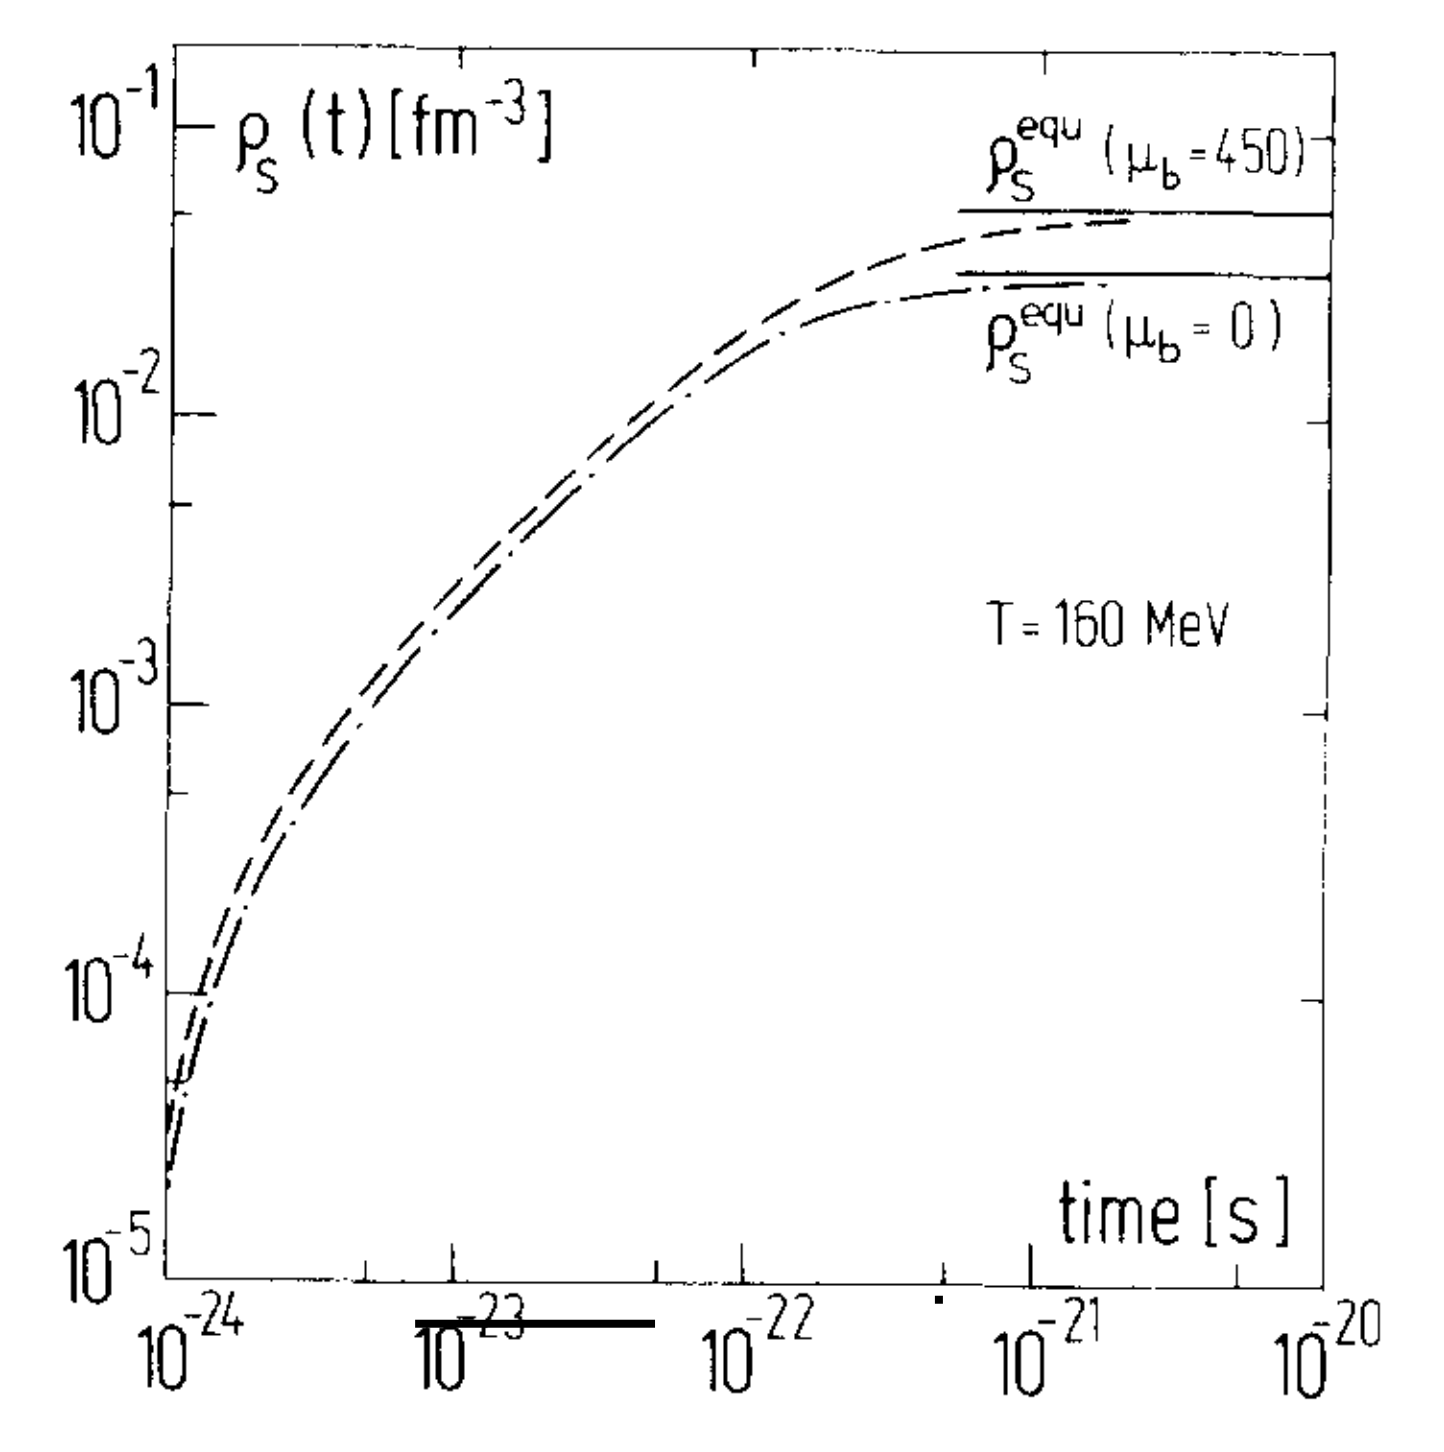
\includegraphics[width=0.38\textwidth]{figures/introduction/hadron_gas_equil.png}
    \caption{The strangeness equilibration time for a QGP (left~\cite{Strangeness}) and a hadronic gas (right~\cite{Strangeness2}) at a temperature of 160 MeV. The QGP can exhibit full chemical equilibration of strangeness in less than $10^{-22}$ seconds, while the hadronic gas takes nearly 100 times longer.}
    \label{fig:qgp_equil}
\end{figure}

\clearpage


\subsubsection{Statistical hadronization}
\label{sec:shm}

The production of strangeness within a system of particles is often described in terms of the \textbf{statistical hadronization model}~\cite{SHM} (SHM). The SHM is based off of the Fermi model of hadron formation, where it is assumed that the strong interactions saturate the quantum particle production matrix elements~\cite{RafelskiSHM}. This assumption allows for the calculation of the particle yields using only conservation laws and the available phase space, while ignoring the unknown microscopic details of the hadronization process. In the fundamental micro-canonical approach for the SHM, the available phase space is determined by the energy density of localized ``clusters'' within the system. However, a grand canonical framework for the SHM is often used for highly energetic systems, where the phase space is determined by a global temperature-like parameter $T$. 

The most important quantity for describing particle yields within the grand canonical SHM is the particle fugacity $\lambda_i$, which is defined as
%
\begin{equation}
    \label{eq:particle_fugacity}
    \lambda_i = e^{\mu_i/T},
\end{equation}
%
where $\mu_i$ is the chemical potential of particle $i$. In essence, the fugacity ``counts'' the number of particles of type $i$ in the system~\cite{Strangeness}. For systems in absolute chemical equilibrium, the chemical potentials for particle and anti-particle flavors are opposite to each other. Consequently, the relationship between the particle and anti-particle fugacities is given by
%
\begin{equation}
    \lambda_{\bar{i}} = \lambda_i^{-1}.
\end{equation}
%
However, this relationship does not hold for systems that have not reached absolute chemical equilibrium, as the chemical potentials of the particle and anti-particle flavors are no longer opposite to each other. Due to the higher mass of the strange quark, the production of $s\bar{s}$ pairs usually proceeds at a much slower rate than the production of $u\bar{u}$ and $d\bar{d}$ pairs. As such, obtaining absolute chemical equilibrium for strange particles is difficult, especially in hadronic matter.\footnote{As mentioned in the previous section, strangeness equilibration in a hadronic gas is over 100 times slower than in the QGP} 

To account for this, the SHM introduces the concept of \textit{relative} chemical equilibrium, in which the strange phase space is not fully saturated, but whatever strangeness is produced is distributed among the strange hadron channels according to the law of maximum entropy~\cite{StrangenessFireball}. The extent to which the strange phase space is saturated is parameterized by $0 < \gamma_s \leq 1$, which gives a modified particle fugacity,
%
\begin{equation}
    \label{eq:modified_fugacity}
    \lambda_i^{\text{mod}} = \gamma_s^{n(i, s)} \lambda_i,
\end{equation}
%
where $n(i, s)$ is the number of strange quarks plus the number of strange anti-quarks in particle $i$. The factor $\gamma_s$ approaches unity whenever the strange phase space is fully saturated (i.e. when the system is in absolute chemical equilibrium). This factor can be determined by looking at strange particle ratios, which are sensitive to the value of $\gamma_s$. For example, the ratio of $\Lambda$ baryons to protons is related to $\gamma_s$ by~\cite{RafelskiSHM}
%
\begin{equation}
    \label{eq:gamma_s}
    \gamma_s^2 = \frac{\Lambda}{\text{p}} \times \frac{\bar{\Lambda}}{\bar{\text{p}}}.
\end{equation}
%

As these particle ratios can be measured by particle collision experiments, it is possible to determine the value of $\gamma_s$ for a given collision system. Measuring $\gamma_s$ in heavy-ion collisions is of particular interest, as it is believed that the QGP is formed in these collisions. However, heavy-ion collisions are very short-lived systems, lasting only around $10^{-23} - 10^{-22}$ seconds~\cite{QGPFormation}. As mentioned previously, full chemical equilibration in a hadronic gas cannot occur within this time frame. As such, measuring large values of $\gamma_s$ in heavy-ion collisions would be a strong indication of QGP formation.

\clearpage

\section{Using Heavy-Ion Collisions to Study the QGP}
\label{sec:heavy_ion_collisions}

As mentioned in Section~\ref{sec:qgp_theory}, there are two ways to transform a hadronic system into the QGP: increasing the system's temperature or increasing its baryon density. Noteably, these two methods are not mutually exclusive: 
\begin{itemize}
    \item Baryon density can be increased by looking at systems with a lot of baryons packed together (like the nucleus of a lead atom)
    \item Temperature can be increased by smashing the aforementioned systems together at higher energies (like in a particle accelerator)
\end{itemize}
Thus one of the best (and only) ways to study the QGP in a laboratory setting is through relativistic \textbf{heavy-ion collisions}: the colliding together of two heavy nuclei at very high energies using a particle accelerator. 

Unfortunately, producing the QGP in this manner has a major drawback; while it is possible to heat up the system beyond the critical temperature required for QGP formation, the system expands and cools \textit{very} quickly. For example, the QGP produced by colliding lead ions with center-of-mass energy \snn = 2.76 TeV at the Large Hadron Collider (LHC) only lasts for around 3 fm/$c$~\cite{QGPFormation}, or $10^{-23}$ seconds. A diagram depicting the formation and evolution of the QGP in a heavy-ion collision can be seen in Figure~\ref{fig:qgp_evolution}. This diagram can be split up into the following stages:
%
\begin{enumerate}
    \item The Lorentz-contracted nuclei approach each other at very high energies, and the partons within the nuclei scatter off each other (t = 0 fm/$c$).
    \item As new partons are created from the initial scatterings, the energy density of the system increases. Eventually this energy density is high enough to create the QGP (t $\approx$ 1 fm/$c$).
    \item Once the QGP is formed, it expands and cools in a hydrodynamic manner. 
    \item After the QGP cools below the critical temperature, the partons begin to hadronize, resulting in the formation of a hadron gas (t $\approx$ 3 fm/$c$).
    \item The hadron gas will continue to expand until the hadrons within the gas are no longer strongly interacting with each other (t $\approx$ 10 fm/$c$). This is often broken up into two stages:
        \begin{itemize}
            \item The hadrons cease to interact \textit{inelastically}, called \textbf{chemical freeze-out}. 
            \item The hadrons cease to interact \textit{elastically}, called \textbf{kinetic freeze-out}.
        \end{itemize} 
    \item The final state hadrons travel outward, where they can be detected experimentally (t $\approx$ $10^{15}$ fm/$c$).
\end{enumerate} 
%
The last stage of this diagram is perhaps the most frustrating: it is only possible to study the QGP by observing the final state hadrons. Luckily, there are some key observables associated with those final state hadrons that can shed light on the formation and evolution of this exciting plasma. Before those observables can be discussed, however, it is necessary to introduce a key concept in heavy-ion collisions: the collision coordinates and the centrality of the collision.

\begin{figure}[ht!]
    \centering
    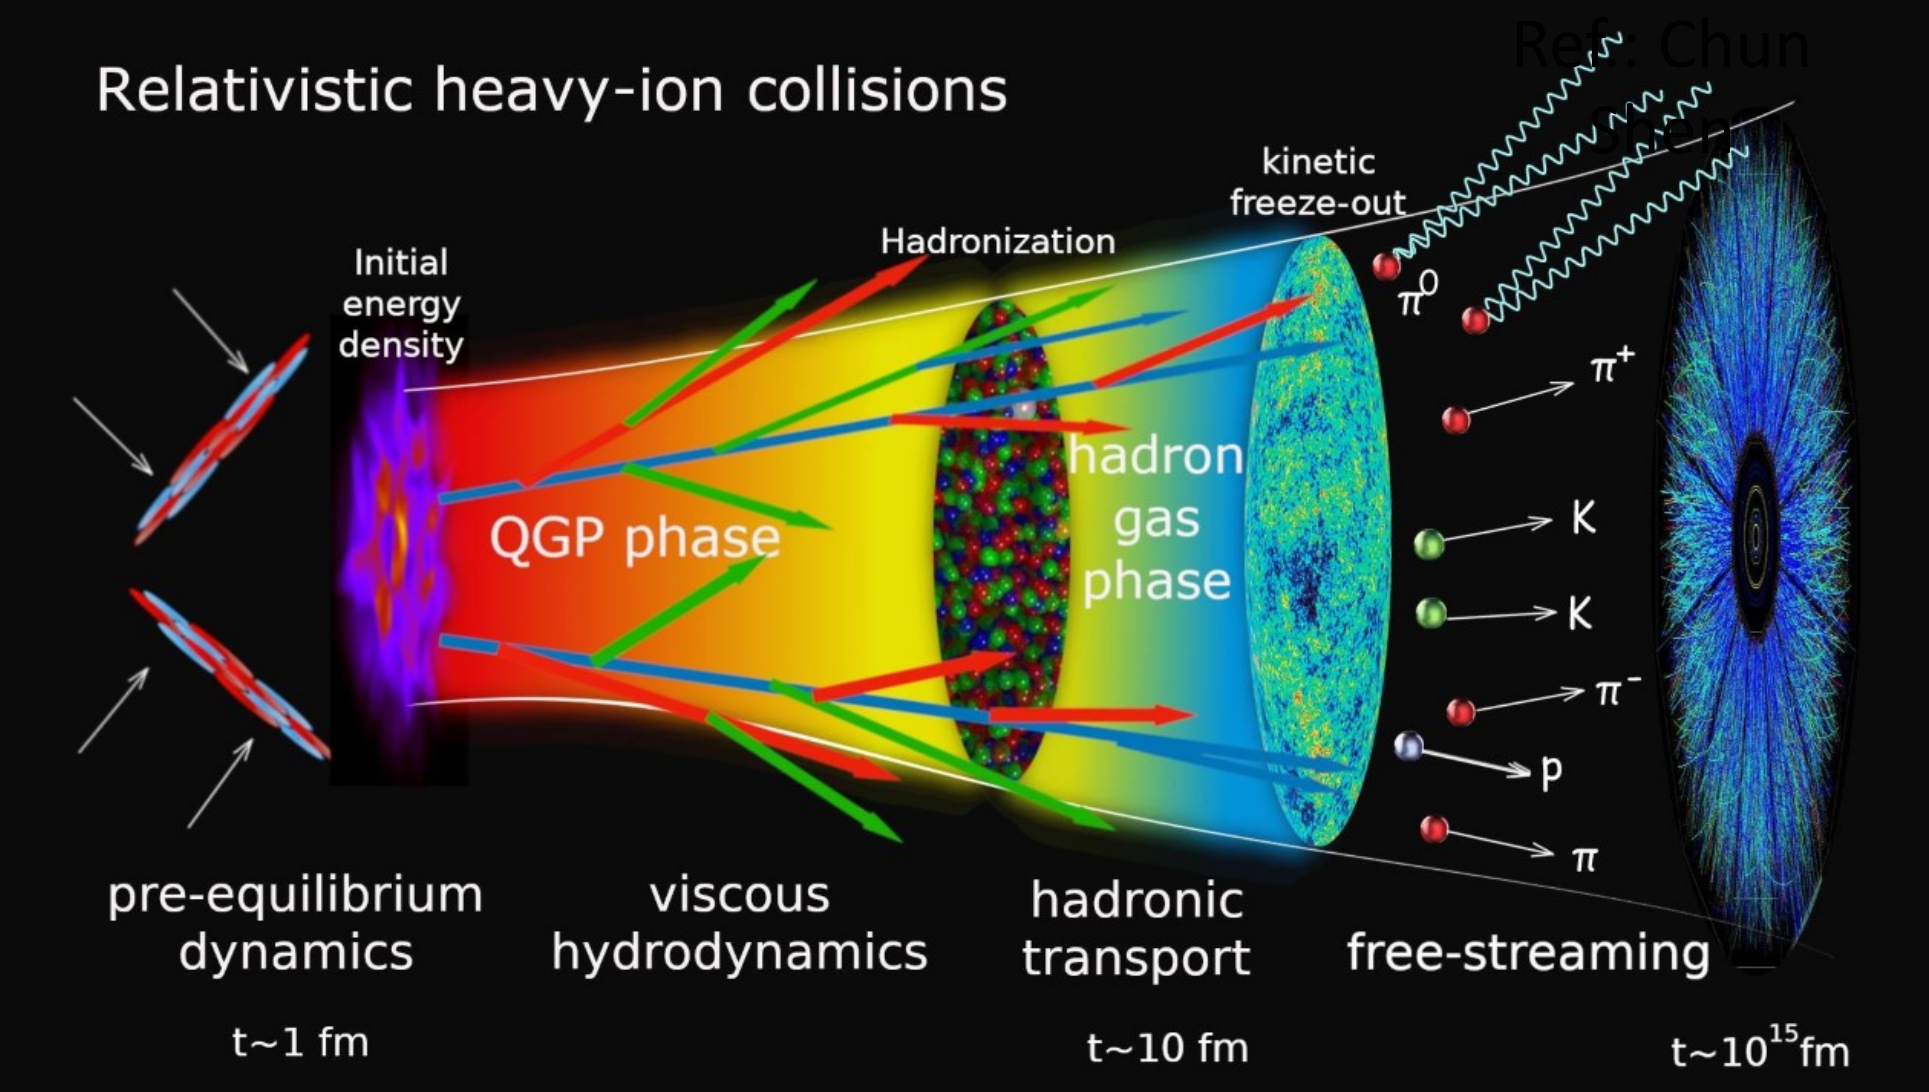
\includegraphics[width=0.8\textwidth]{figures/introduction/heavy_ion_phases.png}
    \caption{A schematic of the formation and evolution of the QGP in a heavy-ion collision. The QGP is formed in the overlap region of the two colliding nuclei, and then expands and cools very quickly.}
    \label{fig:qgp_evolution}
\end{figure}

\subsection{Collision coordinates}
In order to discuss the physics of any collision system, suitable coordinates must be chosen. As many heavy-ion experimental apparatuses are cylinders, the most pragmatic choice is cylindrical coordinates, with the $z$-axis pointing along the beam line. An example of this cylindrical coordinate system is shown in Figure \ref{fig:detector coordinates}. The plane defined by the x- and y-axes is often referred to as the \textbf{transverse plane}, with the angle $\varphi$ referred to as the \textbf{azimuthal angle}.

\begin{figure}
    \centering
    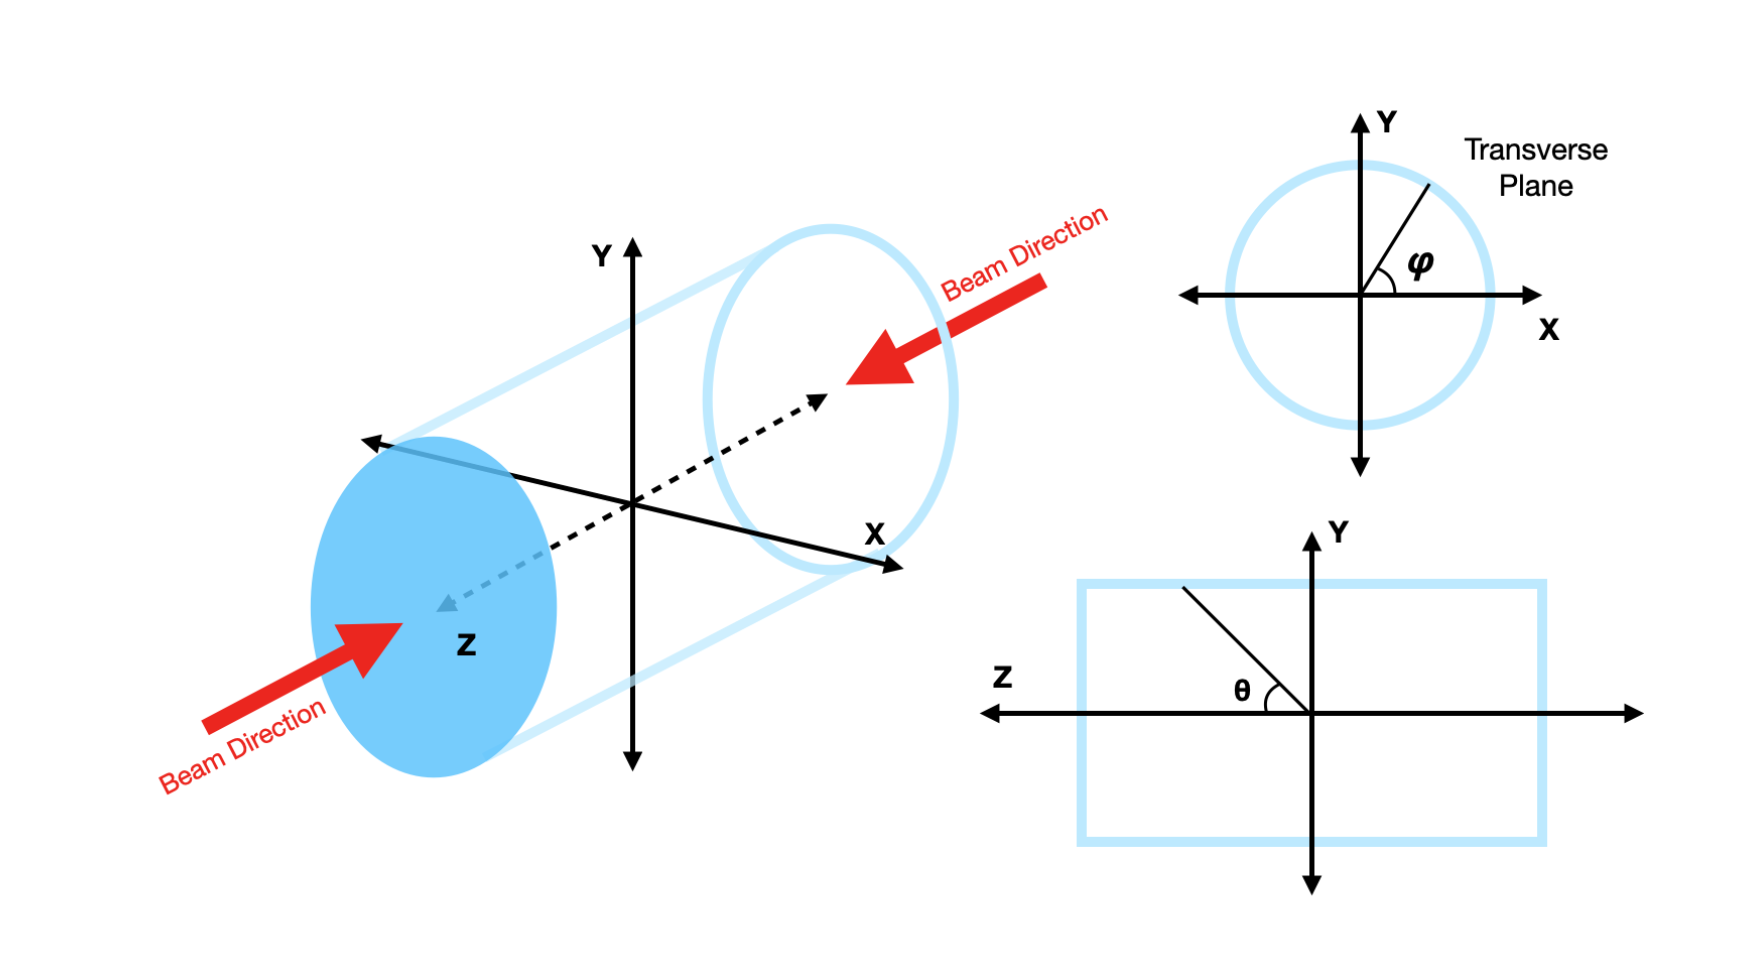
\includegraphics[width=0.8\textwidth]{figures/experiment/detector_coordinates.png}
    \caption{A diagram showing the cylindrical coordinates used to describe particle collision systems.}
    \label{fig:detector coordinates}
\end{figure}

Heavy-ion collisions involve particles moving at relativistic speeds in the beam (z) direction. As such, the polar angle $\theta$ is not particularly useful, as it is not Lorentz invariant. Instead, a more useful quantity is the rapidity $y$, which can be defined as
\begin{equation}
    y = \frac{1}{2} \ln \left( \frac{E + p_{z}}{E - p_{z}} \right),
\end{equation}
where $E$ is the energy of the object being measured and $p_{z}$ is the momentum in the z-direction. This quantity is preferable to $\theta$ as differences in rapidity are invariant under Lorentz boosts along the z-axis. This follows directly from the fact that rapidity is often defined in terms of such boosts,
\begin{equation}
    \left(\begin{array}{c}
        c t^{\prime} \\
        z^{\prime}
        \end{array}\right)=\left(\begin{array}{cc}
        \cosh y & -\sinh y \\
        -\sinh y & \cosh y
        \end{array}\right)\left(\begin{array}{c}
        c t \\
        z
        \end{array}\right) \equiv \Lambda(y)\left(\begin{array}{c}
        c t \\
        z
        \end{array}\right).
\end{equation}
It can be shown\footnote{Using various properties of the hyperbolic trigonometric functions.} that $\Lambda(y)$ obeys
\begin{equation}
    \Lambda(y_1 + y_2) = \Lambda(y_1)\Lambda(y_2),
\end{equation}
which in turn gives a rapidity addition rule for reference frames A, B and C moving along the z-axis,
\begin{equation}
    y_{AC} = y_{AB} + y_{BC}.
\end{equation}
Now suppose reference frame A is the lab (stationary) frame, and reference frames B and C correspond to two different particles. The above equation can then be written as
\begin{equation}
    y_{AC} - y_{AB} = y_{BC} = y_{A'B} - y_{A'C},
\end{equation}
where $A'$ can be \textit{any} reference frame. In other words, the difference in rapidity between any two particles does not depend on the reference frame the measurement is made in. Another consequence of this property is that rapidity distributions of particles do not change shape in different reference frames: they only get shifted along the rapidity axis.

However, the total energy of a given particle is often not known, and thus rapidity is replaced by the more experiment-friendly \textbf{pseudorapidity}, 
\begin{equation}
    \eta = \frac{1}{2} \ln \left( \frac{|\vec{p}| + p_{z}}{|\vec{p}| - p_{z}} \right) 
        = -\ln \left( \tan \frac{\theta}{2} \right),
\end{equation}
where $\theta$ is the aforementioned polar angle. This quantity can be directly measured by experiment, at the expense of losing a small amount of Lorentz invariance: the \textit{pseudo} part of pseudorapidity comes from the idea that at very high momentum ($p >> m$), the rapidity and pseudorapidity are approximately equal.

\subsection{Collision centrality}
\label{sec:collision_centrality}

The very first step of the heavy-ion collision process involves the scattering of the partons within the two nuclei. However, these nuclei are not point-like objects: they have a finite size, and therefore need not collide ``head-on.'' Instead, the nuclei can collide at different \textbf{impact parameters} (commonly denoted as $b$), as shown in Figure~\ref{fig:impact_parameter}. The impact parameter is defined as the distance between the centers of the two nuclei, measured in the transverse plane (the plane perpendicular to the initial directions of the nuclei). Collisions with a large impact parameter give rise to \textit{spectator} nucleons, which do not participate in the collision and continue traveling in the same direction as the initial beams.

\begin{figure}[ht]
    \centering
    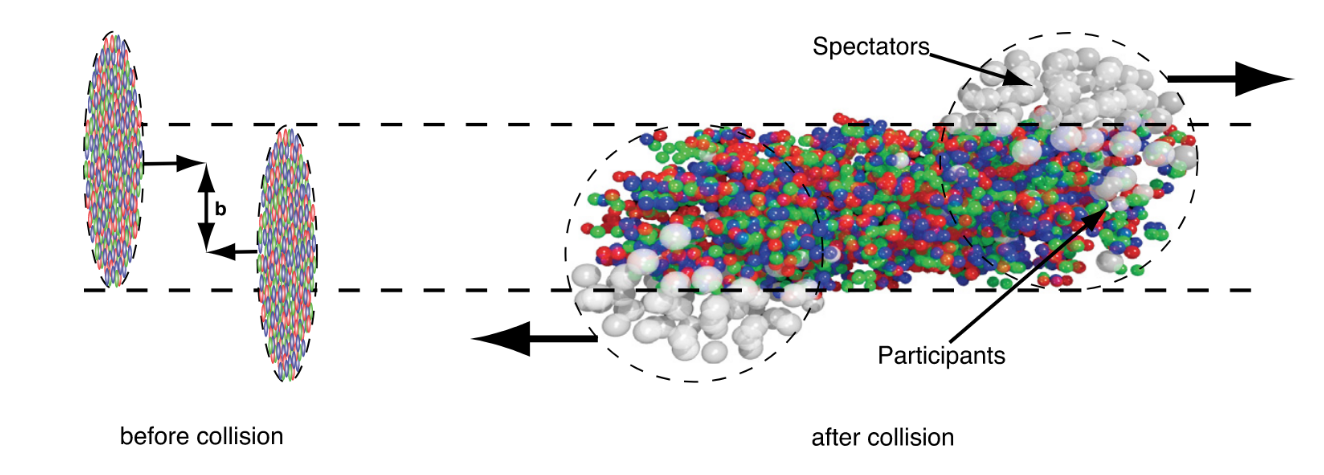
\includegraphics[width=0.9\textwidth]{figures/introduction/impact_parameter.png}
    \caption{A schematic of a heavy-ion collision with impact parameter $b$, taken from~\cite{CERNCourierImpactParam}.}
    \label{fig:impact_parameter}
\end{figure}

The impact parameter is very important when studying the QGP for a fairly straightforward reason: as the impact parameter decreases, the number of partonic scatterings increases, which in turn increases the energy density of the system. In some sense, the size of the impact parameter determines whether or not the QGP is formed in the subsequent stages of the collision. As such, characterizing heavy-ion collisions by their impact parameter is quite useful.  However, the impact parameter is not directly measurable and must be inferred from the final state hadrons.

Instead of classifying collisions based off their unobtainable impact parameter, they can instead be classified by their \textbf{collision centrality}. The collision centrality is defined as
%
\begin{equation}
    \label{eq:centrality}
    c=\frac{\int_0^b d \sigma / d b^{\prime} d b^{\prime}}{\int_0^{\infty} d \sigma / d b^{\prime} d b^{\prime}}=\frac{1}{\sigma_{\mathrm{AA}}} \int_0^b \frac{d \sigma}{d b^{\prime}} d b^{\prime},
\end{equation}
%
where $\sigma_{\mathrm{AA}}$ is the total cross-section of the nucleus-nucleus (A-A) collision. As this number is strictly between 0 and 1, it is often expressed as a percentile: 0\% corresponds to the most central collisions (lowest impact parameters), and 100\% corresponds to the most peripheral collisions (highest impact parameters). If a monotonic relationship between $b$ and the number of final state particles seen in the detector is assumed, the collision centrality can be experimentally determined~\cite{GlauberModelALICE1}. The number of final state particles from a collision is called the \textbf{multiplicity} of the collision, and is often denoted as $N_\text{ch}$. The subscript $ch$ indicates that only charged particles are counted, as neutral particles are not seen by most detectors. 

In practice, the collision centrality percentiles are usually determined by looking at the distribution of events as a function of the signal (effectively $N_\text{ch}$) as measured by a particular detector. The percentile for a specific event can then be determined by integration:
%
\begin{equation}
    \label{eq:centrality_distribution}
    c \approx \frac{1}{\sigma_{A A}} \int_{N_{c h}}^{\infty} \frac{\mathrm{d} \sigma}{\mathrm{d} N_{\mathrm{ch}}^{\prime}} \mathrm{d} N_{\mathrm{ch}}^{\prime},
\end{equation}
%
where $N_\text{ch}$ is the multiplicity of the event in question. An example of separating events into centrality percentiles using this method can be seen in Figure~\ref{fig:alice_centrality}. In this plot, Pb--Pb collisions are characterized by their event activity in the ALICE VZERO detector (which will be discussed in more detail in the next chapter). The red points correspond to fits obtained using Monte Carlo simulations based off of the Glauber model~\cite{GlauberModelALICE1, GlauberModelALICE2}. The Glauber model~\cite{GlauberModel} is a geometric model that treats the nuclei as a collection of nucleons, and models the collisions as a superposition of binary nucleon-nucleon collisions. This model gives a relationship between the impact parameter $b$, the number of participating nucleons $N_{part}$, and the number of binary nucleon-nucleon collisions $N_{coll}$. While not of particular import to this thesis, fitting the Glauber model to the data actually allows for the determination of the impact parameter correponding to a given multiplicity percentile. The fact that the model describes the data well also serves as a sanity check for the experimental estimation of the collision centrality. In this thesis, the terms ``multiplicity percentile'' and ``collision centrality'' will be used interchangeably.

\begin{figure}[t!]
    \centering
    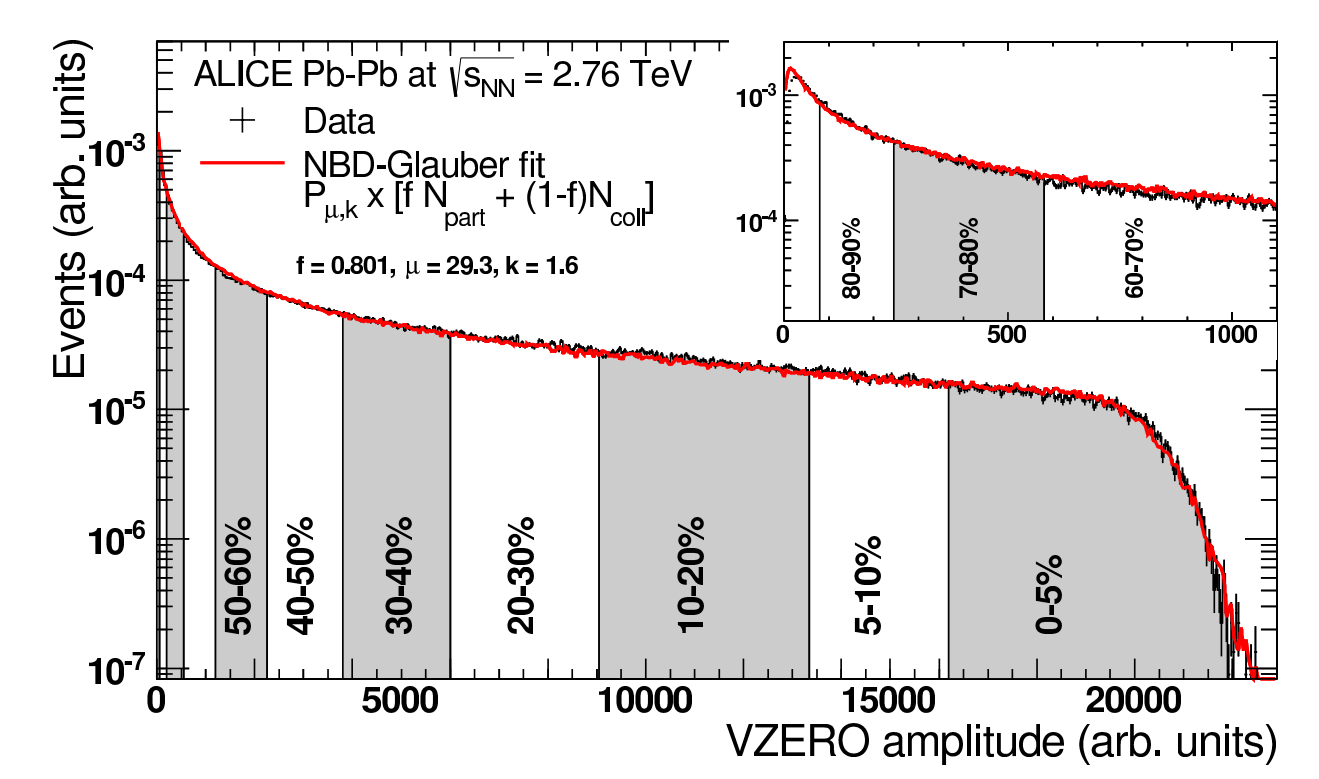
\includegraphics[width=0.9\textwidth]{figures/introduction/alice_centrality.png}
    \caption{The distribution of Pb--Pb collision events as a function of event activity in the ALICE VZERO detector, taken from~\cite{GlauberModelALICE2}.}
    \label{fig:alice_centrality}
\end{figure}

The approximation given by Equation~\ref{eq:centrality_distribution} has an additional benefit: it allows for the classification of the ``size'' of a collision without a clearly defined impact parameter. This is useful for proton-proton and proton-lead collisions, where the impact parameter is ill-defined. 

\subsection{Experimental signatures for QGP formation}
\label{sec:qgp_evidence}

As mentioned in Section~\ref{sec:heavy_ion_collisions}, the QGP produced within a heavy-ion collision is \textit{very} short-lived. As such, any attempt to study the QGP and its formation must be done using the detector-accessible final state hadrons. Luckily, there are a number of experimental signatures associated with the theoretical properties of the QGP discussed in Section~\ref{sec:qgp_properties}. These experimental signatures include:
%
\begin{itemize}
    \item \textbf{jet quenching}~\cite{JetQuenching}, where the energy of a jet is heavily reduced due the radiative energy loss of its constituent partons as they travel through the QGP (Section~\ref{sec:qgp_energy_loss})
    \item \textbf{collective flow}~\cite{CollectiveFlow}, where the fluid-like motion of the partons within the QGP (Section~\ref{sec:qgp_fluid}) results in correlations between the final state hadrons
    \item \textbf{strangeness enhancement}~\cite{Strangeness}, where the enhanced production of strange quarks in the QGP (Section~\ref{sec:qgp_strangeness}) results in an increase in the relative production of strange final state hadrons when compared to non-strange hadrons.
\end{itemize}
%

\subsection{Jet quenching}
\label{sec:jet_quenching}

The high momentum partons produced in the initial hard scatterings of heavy-ion collisions often traverse the QGP medium. Much like electron tomography, where the passage of electrons through an atomic medium can give insight to the structure of the atoms within, high momentum partons can be used to probe the QGP. These colored partons interact with the colored medium, losing energy in the process due to the collisional and radiative processes described in Section~\ref{sec:qgp_energy_loss}. As discussed in Section~\ref{sec:jets}, these partons are never observed individually; instead, they hadronize into a spray of particles known as a jet, which can be measured by the detector. Thus the energy lost by the parton is not observed directly, but rather as a reduction in the energy of the resulting jet. This phenomenon is known as \textbf{jet quenching}, and is one of the most well studied signatures of QGP formation.

Experimentally, this quenching is observed by studying \textit{dijets}. While the term ``jet'' refers to a single spray of particles observed in the detector, the initial hard scattering responsible for the formation of the jet corresponds to the production of \textit{two} high momentum partons. Traveling in opposite directions in the transverse plane, these partons often produce two jets that are back-to-back in $\varphi$ (the azimuthal angle in the transverse plane). These two jets are collectively referred to as a dijet. In pp collisions, the energy of the two jets is roughly equal as the corresponding partons don't lose energy to a medium. In heavy-ion collisions, however, the partons lose energy to the QGP due to gluon radiation and elastic scattering with the medium's constituents~\cite{JetQuenchingReview}. If one of the two partons has a larger path length through the QGP, it will lose more energy than the other parton, resulting in an imbalance in the energy of the two jets. A schematic of this process for pp and A--A collisions can be seen in Figure~\ref{fig:dijet_schematic}. 

However, the path length within the QGP of the dijet-forming partons should be roughly uniform, washing out this assymetry over a large event sample. As such, jet quenching is experimentally observed by selecting high momentum ``trigger'' hadrons, which most likely originated from the parton with the smaller QGP path length. The jet corresponding to this higher momentum trigger--referred to as the ``near-side'' jet--is then compared with its partner jet, which would be $180^\circ$ away in azimuth--called the ``away-side'' jet. The first collaboration to observe this jet quenching was the STAR collaboration at the Relativistic Heavy Ion Collider (RHIC)~\cite{STARJetQuenching}. By looking at high transverse momentum hadrons produced in Au--Au collisions, they found that the away-side jet began to ``disappear'' as the centrality of the collision increased, as shown in Figure~\ref{fig:star_jet_quenching}. This disappearance is due to the away-side jet losing energy to the QGP, such that the corresponding hadrons in the away-side fall below the momentum cutoff.

\begin{figure}[ht]
    \centering
    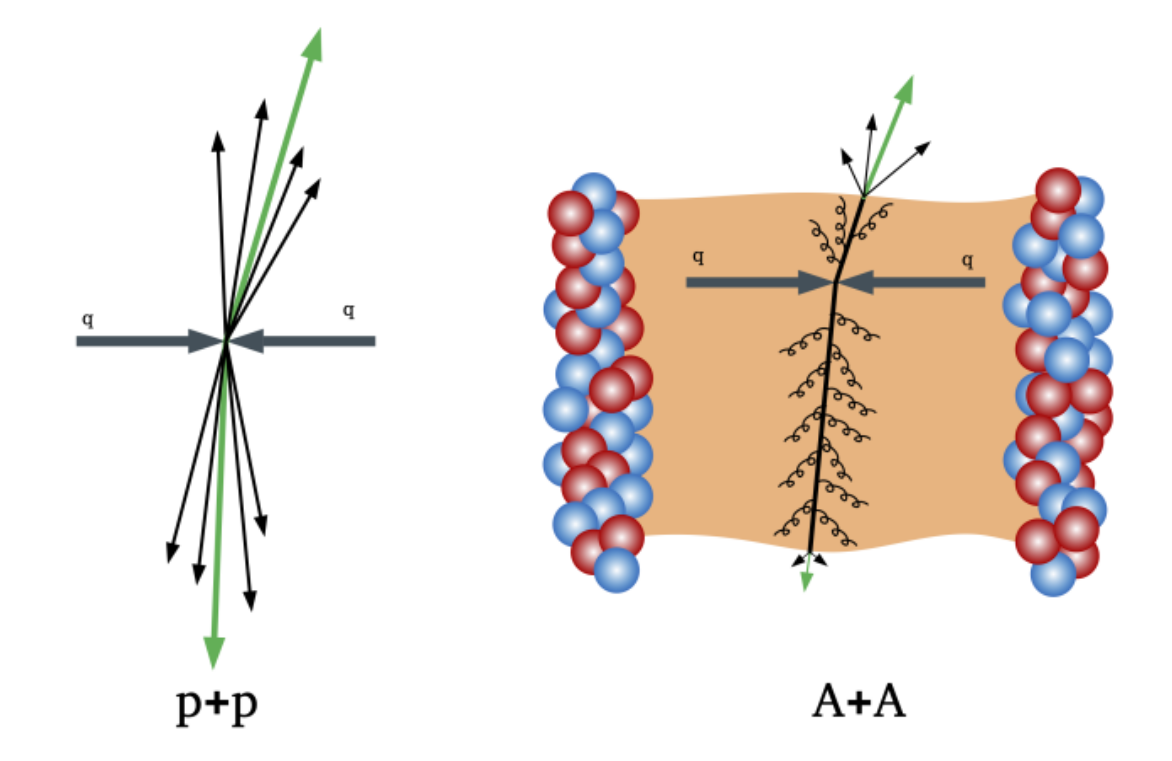
\includegraphics[width=0.7\textwidth]{figures/introduction/dijet_schematic.png}
    \caption{A schematic of the formation of dijets in pp and A--A collisions, taken from~\cite{DijetSchematic}.}
    \label{fig:dijet_schematic}
\end{figure}

\begin{figure}
    \centering
    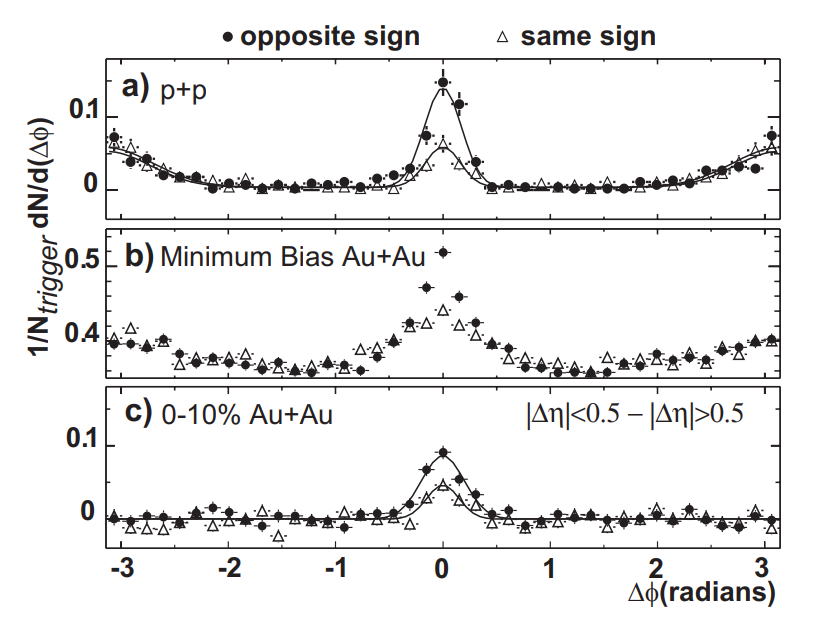
\includegraphics[width=0.7\textwidth]{figures/introduction/star_jet_quenching.png}
    \caption{Hadron yields corresponding to the near-side jet (near $\Delta\varphi = 0$) and the away-side jet ($\Delta\varphi = \pm \pi$), taken from~\cite{STARJetQuenching}. In pp and minimum bias Au--Au collisions, the away-side jet is present. However, at high centrality (0-10\%), the away-side jet completely disappears.}
    \label{fig:star_jet_quenching}
\end{figure}


\clearpage 

\subsection{Collective flow}
\label{sec:collective_flow}

As mentioned in Section~\ref{sec:qgp_fluid}, the QGP is a strongly coupled medium, whose constituent partons are heavily coupled to their surroundings. Just as the pebbles within a river get swept up in the flow of the water, the partons within the QGP are influenced by the flow of this medium. This flow manifests itself by the presence of collective effects in the final state hadrons, which are often quantified using \textbf{collective flow} components. These flow components are obtained by expanding the final state hadron distribution in a Fourier series with respect to the azimuthal angle $\phi$~\cite{Flow24},
%
\begin{equation}
    \label{eq:flow_fourier}
    E \frac{d^3 N}{d^3 p}=\frac{1}{2 \pi} \frac{d^2 N}{p_{\mathrm{t}} d p_{\mathrm{t}} d y}\left(1+\sum_{n=1}^{\infty} 2 v_n \cos \left[n\left(\phi-\Psi_R\right)\right]\right),
\end{equation}
where $E$ is the energy of the particle, $p$ is its momentum, $p_T$ is the momentum component in the plane transverse to the beam axis, $y$ is the particle's rapidity, and $\Psi_R$ is the reaction plane angle. This reaction plane angle is defined by the beam axis and the impact parameter vector. The Fourier coefficients
\begin{equation}
    v_n = \langle \cos[n(\phi - \Psi_R)] \rangle
\end{equation}
determine the ``strength'' of the corresponding flow component. The first two coefficients, $v_1$ and $v_2$, are referred to as \textbf{directed (radial) flow} and \textbf{elliptic flow}, respectively. A non-zero directed flow originates from a longitudinally slanted collision~\cite{DirectedFlow}, and is often much smaller than elliptic flow (by over an order of magnitude)~\cite{DirectedFlow2}. However, it can still effect some of the measurements presented in this thesis (see Section~\ref{sec:radial_flow} for more details).

Elliptic flow characterizes the anisotropy of the particle production in the transverse plane. This anisotropy is believed to be caused by the initial anisotropy of the collision geometry, where the overlap region of the colliding nuclei forms an ``almond'' shape. This almond is where the initial QGP is formed, which then hydrodynamically expands and thermalizes nearly instantaneously. The initial spacial anisotropy results in unequal QGP path lengths for the consituent partons, which ultimately results in an anisotropic momentum distribution for the corresponding hadrons (i.e. partons which travel through more medium lose more energy, as discussed in Section~\ref{sec:jet_quenching}). A diagram depicting this process can be seen in Figure~\ref{fig:elliptic_flow}.

\begin{figure}[ht]
    \centering
    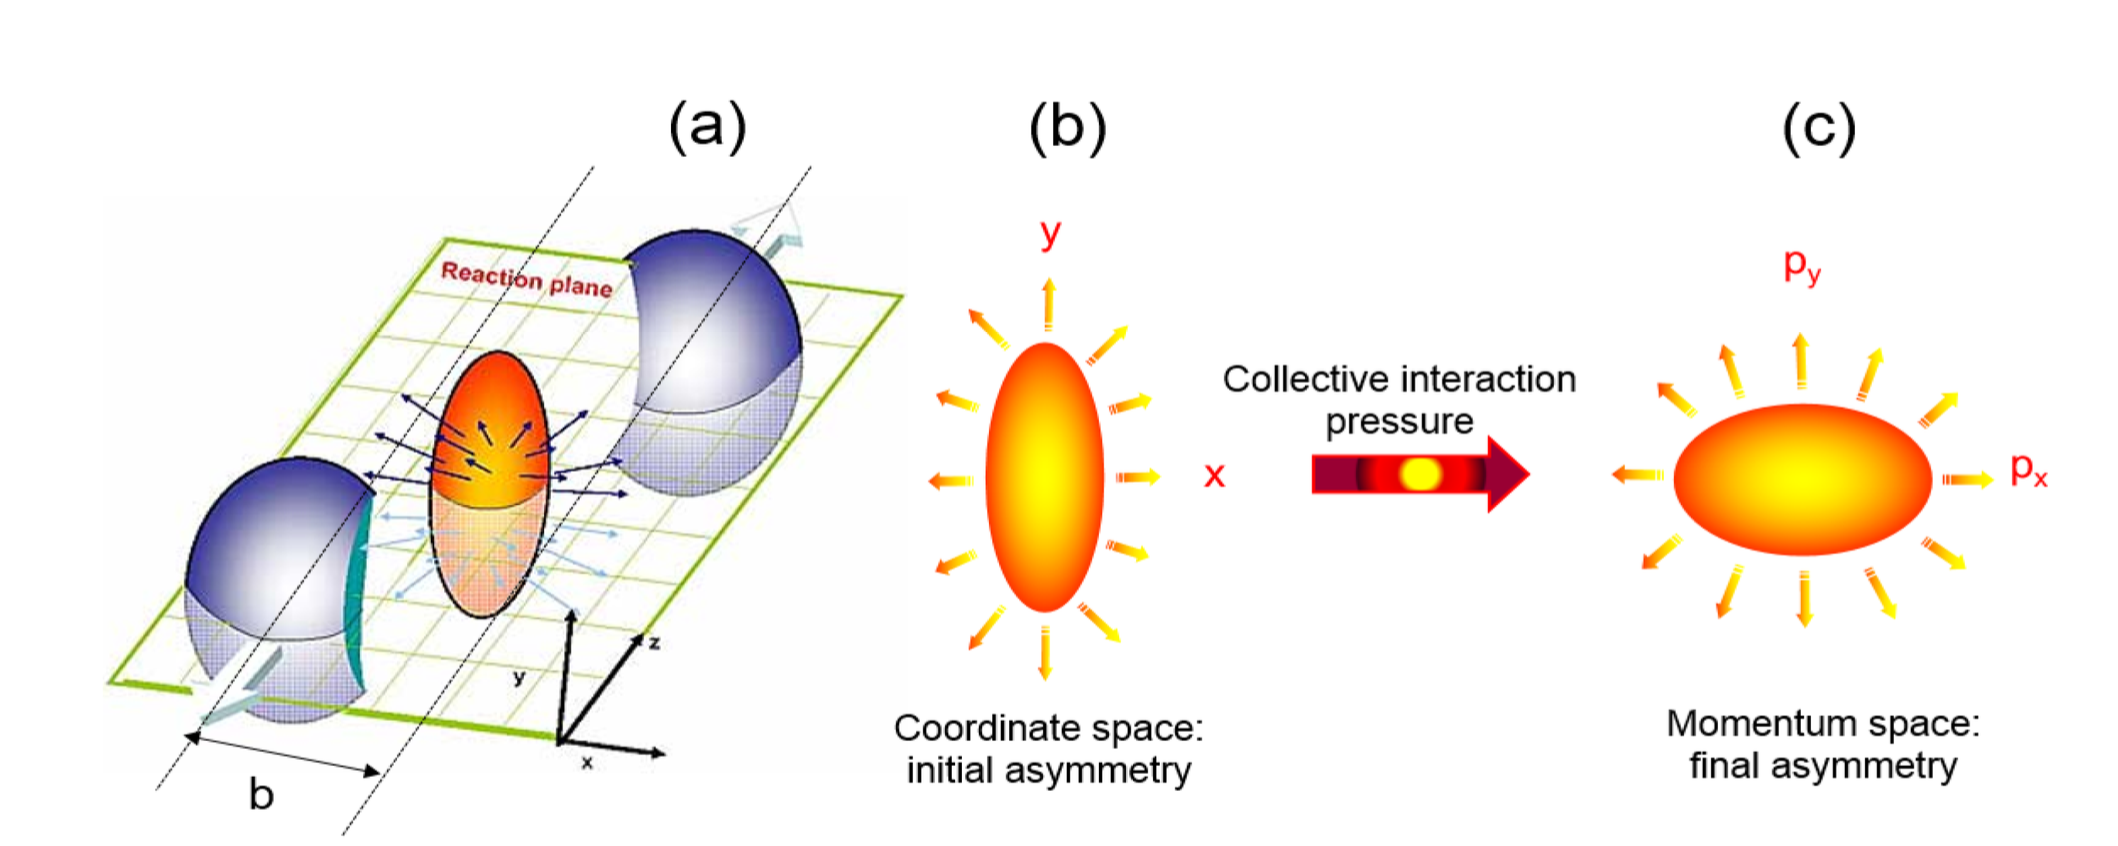
\includegraphics[width=0.9\textwidth]{figures/introduction/elliptic_flow.png}
    \caption{A schematic of the formation of elliptic flow in a heavy-ion collision. The initial anisotropy in coordinate space results in a pressure gradient that causes a momentum space anisotropy in the final state hadrons.}
    \label{fig:elliptic_flow}
\end{figure}


\subsubsection{Measuring flow using two-particle correlations}
\label{sec:v2_twoparticle}
Reconstructing the reaction plane angle $\Psi_R$ is difficult, as it must be done on an event-by-event basis~\cite{Flow24}. As such, it is often more convenient to measure the collective flow components by looking at two-particle correlations in the azimuthal angle $\phi$. In other words, the flow components can be obtained by looking at the distribution of pairs of particles as a function of $\Delta\phi = \phi_1 - \phi_2$, where $\phi_1$ and $\phi_2$ are the azimuthal angles of two (non-identical) particles. This distribution can be decomposed into a Fourier series similar to Equation~\ref{eq:flow_fourier}~\cite{FlowDphi}, 
%
\begin{equation}
    \label{eq:flow_dphi}
    \frac{d N^{\text {pair }}}{d \Delta \varphi}=a_0+2 a_1 \cos \Delta \varphi+2 a_2 \cos 2 \Delta \varphi+\ldots,
\end{equation}
where $v_n \equiv a_n/a_0$ are the very same flow coefficients from before. This bypasses the need to reconstruct the reaction plane angle $\Psi_R$, but it also makes clear that any analyses involving two-particle angular correlations (like the one presented in this thesis) must be mindful of the presence of these coefficients (see Chapter~\ref{ch:analysis_mnm} for more details).

\clearpage

\subsection{Strangeness enhancement}
\label{sec:strangeness_enhancement}

As mentioned in Section~\ref{sec:qgp_strangeness}, strangeness production within the QGP is enhanced relative to a hadronic gas due to the thermal production of strange quarks via gluon fusion. This production mechanism is much faster than strangeness-producing mechanisms within the hadronic gas, allowing for strangeness in the QGP to reach chemical equilibrium within the lifespan of a heavy-ion collision. Thus measuring the extent to which this equilibrium is reached for a given collision system can provide insight into the formation of the QGP.

 Experimentally, the degree of strangeness equilibration is measured by looking at the abundance of strange hadrons relative to non-strange hadrons, like pions. For central heavy-ion collisions--both at the LHC and RHIC--these strange/non-strange particle ratios are found to be consistent with the grand canonical approach to the SHM discussed in Section~\ref{sec:shm}~\cite{NATURE12, NATURE13} with $\gamma_s$ values approaching unity, as seen in Figure~\ref{fig:macro_model}. As mentioned at the end of Section~\ref{sec:shm}, this is a strong indication that the QGP is formed in these collisions. 
 
    \begin{figure}[ht]
        \centering
        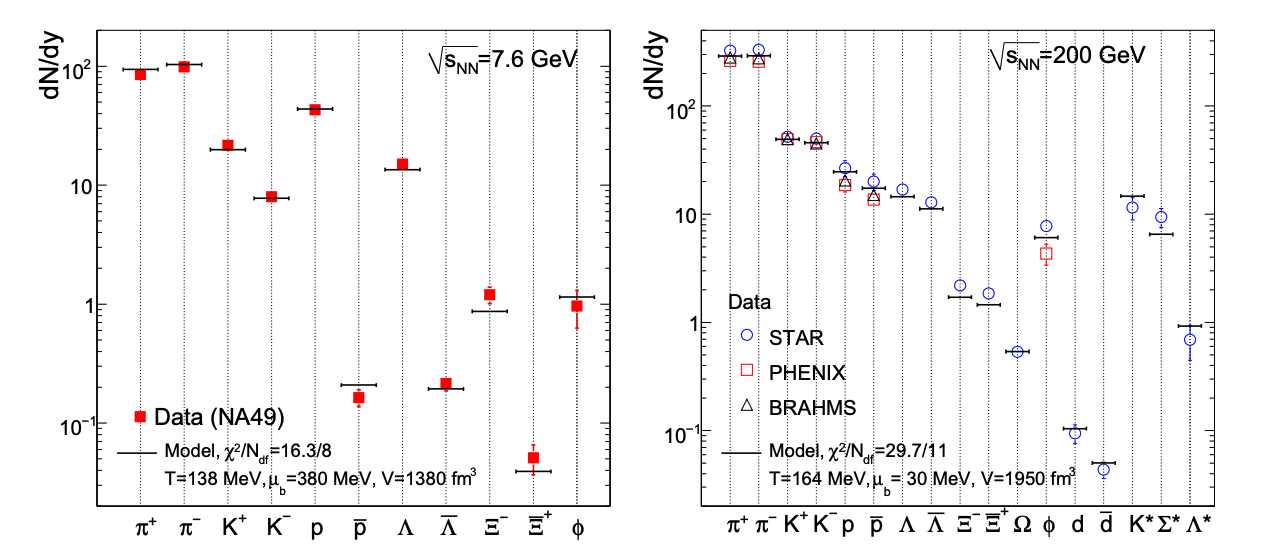
\includegraphics[width=0.9\textwidth]{figures/introduction/macro_model.png}
        \caption{The yields of different hadrons as measured in heavy-ion collisions at \snn = 7.6 GeV (left) and \snn = 200 GeV (right), compared to the grand canonical SHM (black points). In the lower energy collision, the temperature (138 MeV) is well below the critical temperature for QGP formation, and chemical equilibration is not reached ($\gamma_s \approx 0.6$) (found by Equation~\ref{eq:gamma_s}). In the higher energy collision, the temperature is high enough for QGP formation, and chemical equilibration is nearly reached ($\gamma_s \approx 1$). Taken from~\cite{NATURE12}.}
        \label{fig:macro_model}
    \end{figure}

    \clearpage
 
 
 The particle ratios as measured in lower multiplicity pp collisions at the LHC are also found to be consistent with the grand canonical SHM \textit{without} chemical equilibriation~\cite{NATURE14, NATURE15}, with a measured $\gamma_s \approx 0.6$ across a wide range of values for the collision energy, as shown in Figure~\ref{fig:micro_model}. Under the strangeness enhancement picture, this indicates that QGP formation does \textit{not} occur in these lower multiplicity pp collisions. 

\begin{figure}[ht]
    \centering
    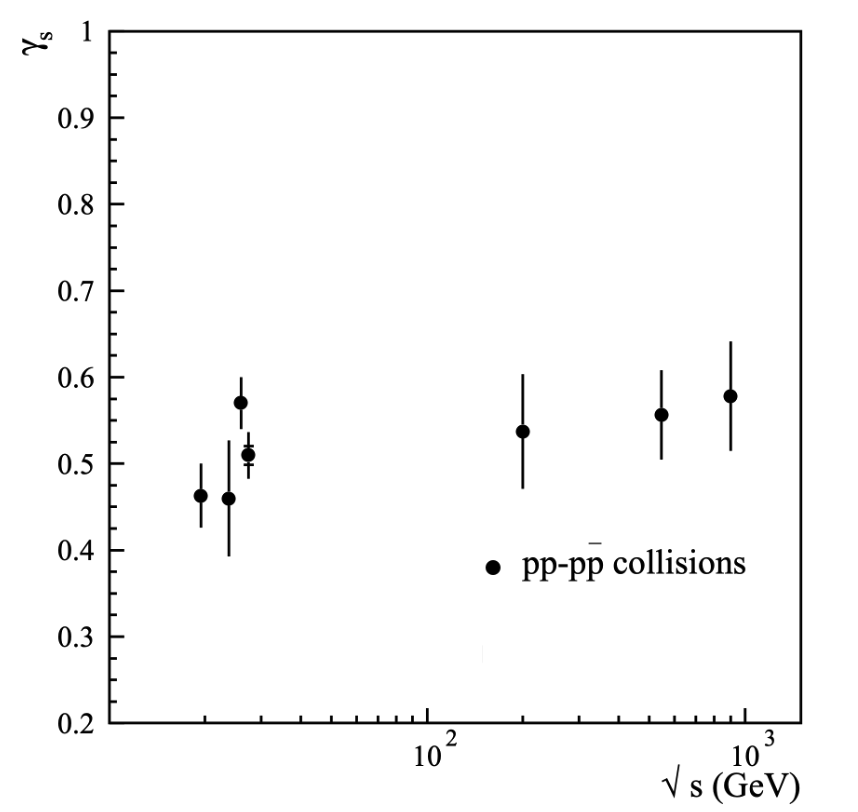
\includegraphics[width=0.6\textwidth]{figures/introduction/micro_model.png}
    \caption{The measured values of $\gamma_s$ in low multiplicity pp collisions across a wide range of collision energies ($\sqrt{\text{s}}4$). The extracted temperatures (under the grand canonical SHM model) are greater than 160 MeV for each reported energy. As $\gamma_s$ is much less than unity, the chemical equilibration of strangeness is nowhere near being reached. Taken from~\cite{NATURE14}.}
    \label{fig:micro_model}
\end{figure}

 \subsubsection{Strangeness in small systems: is the QGP formed?}

 Filling in the gaps between low multiplicity pp collisions and high multiplicity Pb--Pb collisions reveals a complicated picture, as shown in Figure~\ref{fig:strangeness_enhancement}. The strange/non-strange particle ratios seem to be consistent with a smooth transition between the two regimes, independent of the collision system. In other words, the ratios in higher multiplicity pp and p--Pb collisions match up nicely with the ratios in lower multiplicity Pb--Pb collisions. This indicates that the enhanced production of strange quarks is not exclusive to heavy-ion collisions; there is an ``onset'' of strangeness enhancement occuring in lower multiplicity pp and p--Pb collisions. Furthermore, this enhancement is seen to scale with the number of strange quarks in the hadron: the $\Omega$ baryon ($sss$) exhibits the largest enhancement, while the proton ($uud$) sees virtually no increase. 
 
 \begin{figure}
    \centering
    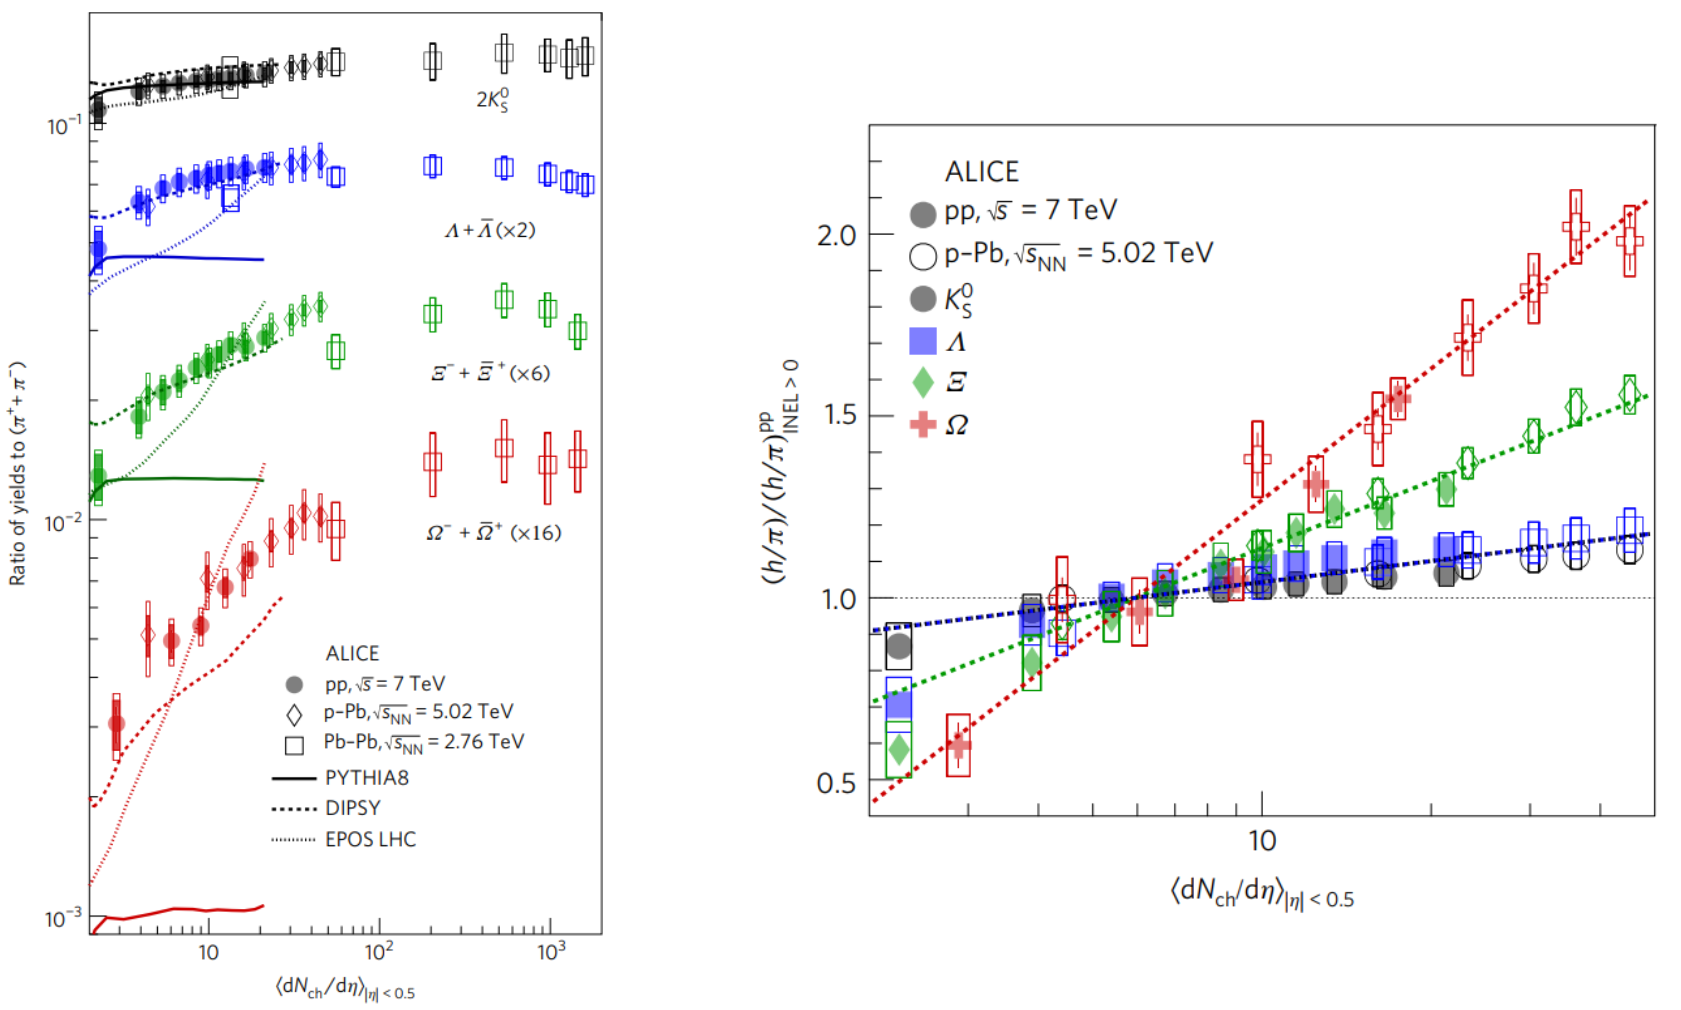
\includegraphics[width=0.9\textwidth]{figures/introduction/strangeness_enhancement.png}
    \caption{The particle ratios of strange hadrons to pions as a function multiplicity for different collision systems (left) and those same ratios normalized to an inclusive pp sample (right). The ratios appear to only depend on the multiplicity of the collision, and not the collision system. Taken from~\cite{NATURE}.}
    \label{fig:strangeness_enhancement}
\end{figure}

As discussed in Section~\ref{sec:qgp_strangeness}, the equilibration of strangeness within a hadronic gas is orders of magnitude slower than the equilibration within the QGP. As such, the onset of strangeness enhancement (which can be viewed as an onset of a full chemical equilibration) in these smaller collision systems can only be explained by the formation of QGP.\footnote{Or, at the very least, smaller QGP-like droplets that exhibit similar thermal strange quark production.} While extensions to the aforementioned statistical models can describe these multiplicity-dependent particle ratios in a phenomenological manner~\cite{NATURE17}, the microscopic origins of this enhancement are not well understood. By investigating the production of strange hadrons in p--Pb collisions (where the onset is greatest), this thesis aims to shed light on the origins of this strange enhancement. However, it is necessary to first introduce some theoretical models to help interpret the results of this thesis.


\section{Simulating Heavy-Ion Collisions}
\label{sec:models}

Theoretical models of heavy-ion collisions are necessary for the understanding of QCD and the QGP. Without them, there would be no framework for interpreting the results from the experiments dedicated to studying this strongly interacting plasma. Unfortunately, due to the complexity of these heavy-ion collision systems, there is no \textit{single} model that can describe the entire collision evolution. Instead, the choice of model to compare a particular observable to depends very heavily on the observable in question. For example, some models treat the QGP phase of the collision as a hydrodynamic system, washing out information about the initial partonic scatterings~\cite{EPOS}. This can be useful when trying to study bulk properties of the QGP (like the $v_2$ from Section~\ref{sec:collective_flow}), but not-so-useful when studying jets and their consituents. Other models focus more on the individual partonic scatterings and subsequent hadronization, but do not include an explicit QGP phase~\cite{Pythia, DPMJet}. Such models are powerful tools for analyzing smaller collision systems (pp and lower multiplicity p--Pb), but fail to capture many of the features observed in heavy-ion collision data. In this section, the models used to help interpret the results of this thesis will be discussed. All of these models are capable of simulating pp, p--Pb, and Pb--Pb events.

\subsection{PHSD}
Parton-Hadron-String-Dynamics (PHSD)~\cite{PHSD1, PHSD2} is the only model explored in this thesis that utilizes a \textbf{microscopic transport approach}: it simulates the full space-time evolution of a heavy-ion collision by modeling the interactions of individual particles. Here ``particles'' refers to different quantities (strings, partons, hadrons) which are all evolved in different ways. The transport equations of the partons and hadrons are derived from the Kadanoff-Baym (KB) equations~\cite{KBEq}, which describe the non-perturbative transport of particles in a strongly interacting system. The evolution of a collision within PHSD is described in the following sections.

\subsubsection{Initial stages}
Prior to the collision, the simulation is broken up into a 3D-grid of size 56 in each of the x, y, and z directions. The total size of the grid increases with each time step such that the number of particles within a given cell evolves smoothly with time. The initial momentum distribution and abundances of partons within the nuclei (prior to any collision) are given by the thermal distributions
\begin{equation}
    f(\omega, \vec{p}) = C_i p^2 \omega \rho_i(\omega, \vec{p}) n_{F / B}(\omega / \tau),
\end{equation}
where $\rho_i$ are the spectral functions of the quarks and gluons ($i = q, \bar{q}, g$) and $n_{F / B}$ are the Fermi-Dirac (for quarks) and Bose-Einstein (for gluons) distributions. Once the nuclei collide, the partons interact with each other under the Lund string model to form \textit{leading hadrons} (at large rapidity) and \textit{pre-hadrons} (at midrapidity), as shown in Figure~\ref{fig:lund_string_phsd}. The leading hadrons are immune to dissociation within the QGP, while the pre-hadrons are not. 

\begin{figure}[ht]
    \centering
    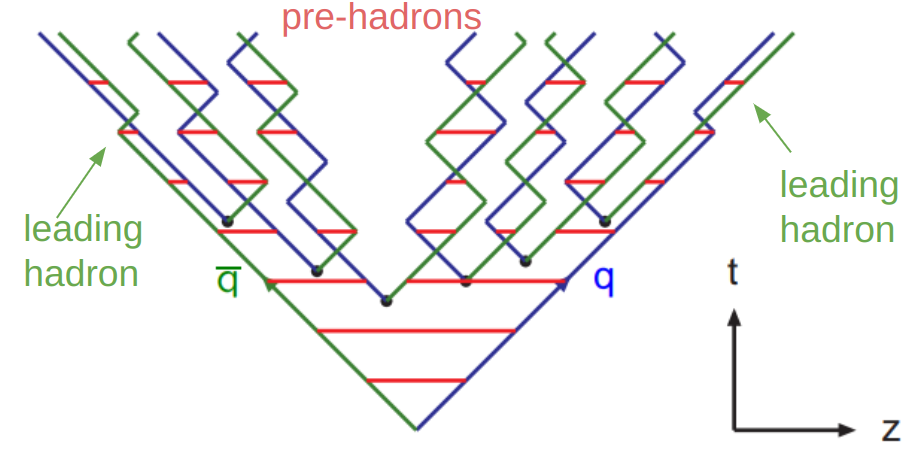
\includegraphics[width=0.5\linewidth]{figures/introduction/lund_string_phsd.png}
    \caption{The Lund string model, with pre-hadrons and leading hadrons labeled.}
    \label{fig:lund_string_phsd}
\end{figure}

\subsubsection{QGP phase}
If the energy density $\epsilon$ of a given cell increases beyond the critical energy density $\epsilon_c = 0.5$ GeV/fm$^3$, the pre-hadrons within that cell are dissolved into partons. The partons are then treated as interacting quasi-particles under the DQPM~\cite{DQPM} model, with Lorentzian spectral functions given by
\begin{equation}
\rho_j(\omega)=\frac{\gamma_j}{E_j}\left(\frac{1}{\left(\omega-E_j\right)^2+\gamma_j^2}-\frac{1}{\left(\omega+E_j\right)^2+\gamma_j^2}\right)
\end{equation}
where $i$ is one of $(q, \bar{q}, g)$ and the width $\gamma_i$ is given by
\begin{equation}
\gamma_g(T)=N_c \frac{g^2 T}{8 \pi} \ln \frac{2 c}{g^2}, \quad \gamma_q(T)=\frac{N_c^2-1}{2 N_c} \frac{g^2 T}{8 \pi} \ln \frac{2 c}{g^2},
\end{equation}
where $T$ is the temperature (calculated from the energy density within a given cell). This is the key difference between DQPM and other transport models--the quarks and gluons have non-zero temperature-dependent widths in the medium! The coupling constant $g$ is also temperature dependent, and is of the form
\begin{equation}
    g^2\left(T / T_c\right)=\frac{48 \pi^2}{\left(11 N_c-2 N_f\right) \ln \left(\lambda^2\left(T / T_c-T_s / T_c\right)^2\right.}.
\end{equation}
The parameters $T_s$ and $\lambda$ are fit to lQCD results~\cite{PHSD2}. The spectral functions are enough to describe the propagation of the mean-fields of the partons (effectively their Green's functions) via the aforementioned KB equations. The collisional terms in these equations are determined by the modified scattering cross-sections of the partons. These cross-sections are calculated using the leading order Feynman diagrams, with the DQPM-modified quark and gluon propagators given by
\begin{equation}
    i \delta_{i j} \frac{q+M_q}{q^2-M_q^2+2 i \gamma_q q_0}
\end{equation}
and
\begin{equation}
    -i \delta_{a b} \frac{g^{\mu \nu}-q^\mu q^\nu / M_g^2}{q^2-M_g^2+2 i \gamma_g q_0},
\end{equation}
respectively. Due to the large masses of the gluons, $q + \bar{q} \rightarrow g + g$ and $g \rightarrow g + g$ are suppressed and thus not included in the model.

\subsubsection{Hadronization}
Whenever the energy density of a given cell falls below the aforementioned critical energy density ($\epsilon_c = 0.5$ GeV/fm$^{3}$), the partons within begin to hadronize. The dynamical hadronization of partons into hadrons is modeled by the equations
%
\begin{equation}
\label{eq:meson_hadronization}
\begin{aligned}
& \frac{d N_m(x, p)}{d^4 x d^4 p}=\operatorname{Tr}_q \operatorname{Tr}_{\bar{q}} \delta^4\left(p-p_q-p_{\bar{q}}\right) \delta^4\left(\frac{x_q+x_{\bar{q}}}{2}-x\right) \\
& \quad \times \omega_q \rho_q\left(p_q\right) \omega_{\bar{q}} \rho_{\bar{q}}\left(p_{\bar{q}}\right)\left|v_{q \bar{q}}\right|^2 W_m\left(x_q-x_{\bar{q}},\left(p_q-p_{\bar{q}}\right) / 2\right) \\
& \quad \times N_q\left(x_q, p_q\right) N_{\bar{q}}\left(x_{\bar{q}}, p_{\bar{q}}\right) \delta(\text { flavor, color }) .
\end{aligned}
\end{equation}
%
for mesons and 
%
\begin{equation}
\label{eq:baryon_hadronization}
\begin{aligned}
& \frac{d N_B(x, p)}{d^4 x d^4 p}=\operatorname{Tr}_{q_1} \operatorname{Tr}_{q_2} \operatorname{Tr}_{q_3} \delta^4\left(p-p_{\xi_3}\right) \delta^4\left(x-\xi_3\right) \delta\left(\sqrt{\left(\tau_1-\tau_2\right)^2}\right) \\
& \quad \times \omega_{q_1} \rho_{q_1}\left(p_1\right) \omega_{q_2} \rho_{q_2}\left(p_2\right) \omega_{q_3} \rho_{q_3}\left(p_3\right) \\
& \quad \times\left|M_{q q q}\right|^2 W_B\left(\xi_1, \xi_2, p_{\xi_1}, p_{\xi_2}\right) \\
& \quad \times N_{q_1}\left(x_1, p_1\right) N_{q_2}\left(x_2, p_2\right) N_{q_3}\left(x_3, p_3\right) \delta \text { (flavor, color). }
\end{aligned}
\end{equation}
for baryons. The terms for the meson case are described as follows:
\begin{itemize}
    \item $\text{Tr}_q$ is shorthand notation for $\operatorname{Tr}_q=\sum_q \int d^4 x_q \int \frac{d^4 p_q}{(2 \pi)^4}$, where $q$ is summed over all spin, color, and flavor degrees of freedom.
    \item $\delta^4(p-p_q-p_{\bar{q}})$ forces conservation of four-momentum. Note that the quarks and anti-quarks are allowed to be off-shell (due to their non-zero widths), thus this can result in off-shell mesons.
    \item $\delta^4\left(\frac{x_q+x_{\bar{q}}}{2}-x\right)$ puts the resulting meson in-between the quark and anti-quark pair.
    \item $\omega_q$ and $\omega_{\bar{q}}$ are the energies of the quark and anti-quark, respectively.
    \item $\rho_q\left(p_q\right)$ and $\rho_{\bar{q}}\left(p_{\bar{q}}\right)$ are the aforementioned spectral functions of the quark and anti-quark, respectively.
    \item $\left|v_{q \bar{q}}\right|^2$ is the DQPM-determined \textit{effective quark-anti-quark interaction}, which is shown as the green dashed line in Figure~\ref{fig:vqq}. Note that this value is very small for large quark (energy) densities, and thus this entire equation is effectively zero. However, for low quark densities this value blows up, which ``turns on'' the hadronization (and also guarantees that all partons will hadronize \textit{eventually}).
    \item $W_m\left(x_q-x_{\bar{q}},\left(p_q-p_{\bar{q}}\right) / 2\right)$ is the phase-space distribution of the resulting pre-meson
    \item $N_q\left(x_q, p_q\right)$ and $N_{\bar{q}}\left(x_{\bar{q}}, p_{\bar{q}}\right)$ are the phase-space densities of the quark and anti-quark, respectively.
    \item $\delta(\text { flavor, color })$ represents the function responsible for ensuring flavor quantum numbers are conserved, and that the resulting hadron is color neutral.
\end{itemize}
The terms for the baryon case are similar.

\begin{figure}[ht]
    \centering
    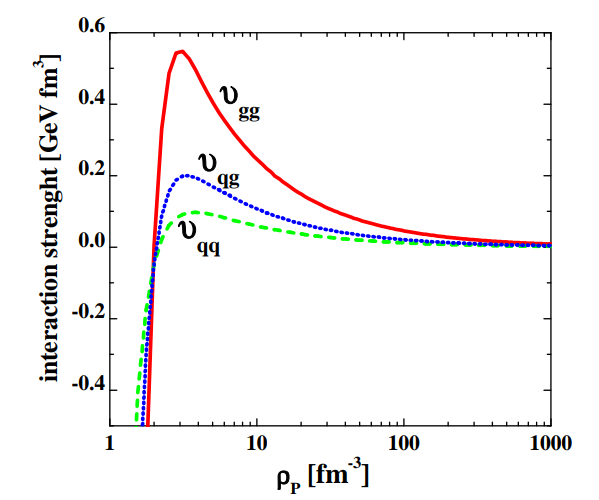
\includegraphics[width=0.5\linewidth]{figures/introduction/vqq.png}
    \caption{The effective quark-quark (green), quark-gluon (blue), and gluon-gluon (red) interactions as a function of parton density in DQPM, taken from~\cite{PHSD1}.}
    \label{fig:vqq}
\end{figure}

The numerical integrations of equations \ref{eq:meson_hadronization} and \ref{eq:baryon_hadronization} for a fixed test parton ultimately give the probability for a hadronization event to occur. From there, events are randomly selected using Monte Carlo techniques, which give a color neutral state with definite x, p and flavor. However, this is \textit{still} not enough to specify a hadron completely: many hadronic states of the same flavor have large widths. Thus to determine the identity of the final hadron, the weight of each possible\footnote{PHSD only includes the baryon octet/decouplet, the spin 0 and spin 1 meson nonets, and a few higher resonance states. Furthermore, if the invariant mass of the color neutral state is above 1.3 GeV (for mesons) or 1.5 GeV (for baryons), the state is treated as a Lund string with further decay handled by the JETSET algorithm~\cite{JETSET}} hadronic spectral function is computed. The hadron is then randomly assigned an identity based on these weights using Monte Carlo.

\subsubsection{Hadronic phase}
All of the hadrons produced in the previous steps are transported using Hadron-String-Dynamics~\cite{HSD} (HSD). The phase-space distributions of the hadrons in HSD are transported using the equation
\begin{equation}
\label{eq:hadron_transport}
\begin{aligned}
& \left\{\left(\Pi_\mu-\Pi_\nu \partial_\mu^p U_{\mathrm{h}}^\nu-M_{\mathrm{h}}^* \partial_\mu^p U_{\mathrm{h}}^{\mathrm{S}}\right) \partial_x^\mu+\left(\Pi_\nu \partial_\mu^x U_{\mathrm{h}}^\nu+M_{\mathrm{h}}^* \partial_\mu^x U_{\mathrm{h}}^{\mathrm{S}}\right) \partial_p^\mu\right\} f_{\mathrm{h}}(x, p) \\
& =\sum_{\mathrm{h}_2 \mathrm{~h}_3 \mathrm{~h}_4 \ldots} \int d 2 d 3 d 4 \ldots\left[G^{\dagger} G\right]_{12 \rightarrow 34 \ldots} \delta_{\Gamma}^4\left(\Pi+\Pi_2-\Pi_3-\Pi_4 \ldots\right) \\
& \times\left\{f_{\mathrm{h}_3}\left(x, p_3\right) f_{\mathrm{h}_4}\left(x, p_4\right) \bar{f}_{\mathrm{h}}(x, p) \bar{f}_{\mathrm{h}_2}\left(x, p_2\right)\right. \\
& \left.-f_{\mathrm{h}}(x, p) f_{\mathrm{h}_2}\left(x, p_2\right) \bar{f}_{\mathrm{h}_3}\left(x, p_3\right) \bar{f}_{\mathrm{h}_4}\left(x, p_4\right)\right\} \ldots,
\end{aligned}
\end{equation}
where $U_h^S$ and $U_h^\mu$ are the scalar and vector hadron self-energies, respectively. The effective mass of the hadron $M_h^*$ is given by
\begin{equation}
    M_h^* = M_h + U_h^S,
\end{equation}
and its effective momentum is given by
\begin{equation}
    \Pi^\mu = p^\mu - U_h^\mu.
\end{equation}
The ``collisional'' term $\left[G^\dagger G\right]_{12 \rightarrow 34 \ldots}$ is the transition rate for the process $1 + 2 \rightarrow 3 + 4 + \ldots$, which is modeled using Lund string fragmentation. The self-energies $U_h^S$ and $U_h^\mu$ are evaluated on the basis of a Nambu-Jona-Lasinio (NJL)-type model~\cite{NJL} for the QCD Lagrangian. Once these self-energies (and $\left[G^\dagger G\right]_{12 \rightarrow 34 \ldots}$) are specified, the transport equation (Equation ~\ref{eq:hadron_transport}) can be solved.

\subsubsection{A simple overview}
While the equations that govern PHSD are quite complicated, the overall picture is relatively simple. It can be summarized as follows:
\begin{itemize}
    \item First, the simulation is split up into cells whose sizes evolve with time, as shown in Figure~\ref{fig:phsd_cells}.
    \item As the initial nuclei collide, and the interacting partons form pre-hadrons and leading hadrons.
    \item If the energy density of a cell is too high, the pre-hadrons dissolve into partons, which are handled by the DQPM model.
    \item If a cell with partons in it cools off, the partons dynamically hadronize.
    \item The resulting hadrons (and any hadrons present in a particular cell) are transported using HSD.
\end{itemize}

\begin{figure}
    \centering
    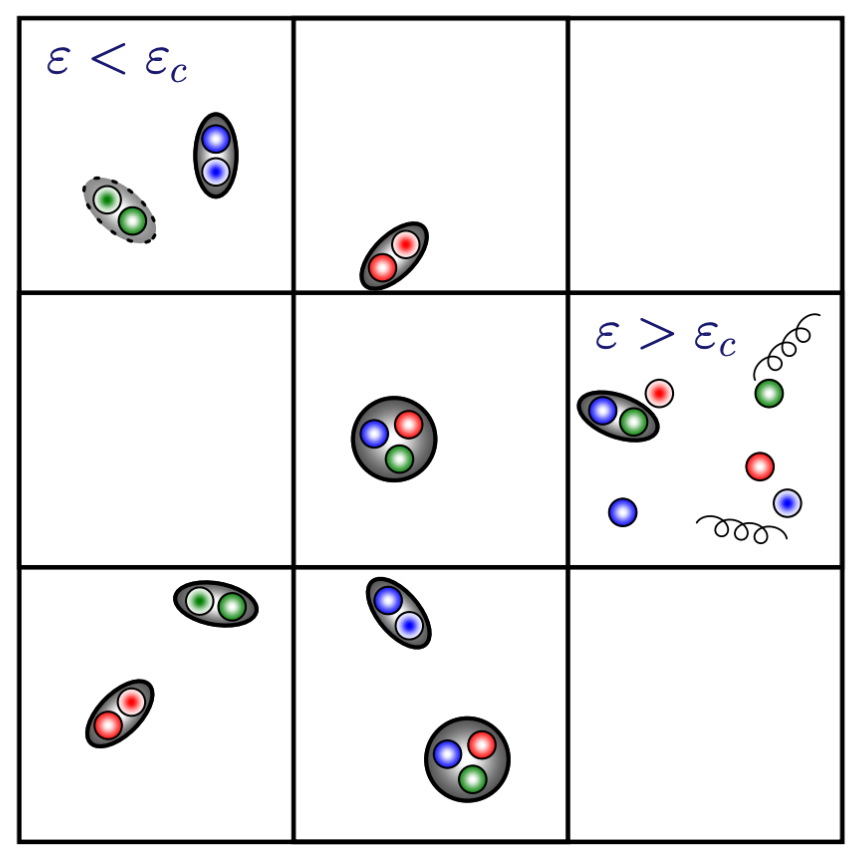
\includegraphics[width=0.5\linewidth]{figures/introduction/phsd_cells.png}
    \caption{The cells within PHSD. If the energy density of the cell is greater than the critical energy density, the pre-hadrons dissolve into partons.}
    \label{fig:phsd_cells}
\end{figure}

\subsection{EPOS LHC}

Another model used to simulate heavy-ion collisions is the EPOS LHC~\cite{EPOSLHC} model. In this model, the initial colliding nuclei results in many parton-parton scatterings happening in parallel, as shown in Figure~\ref{fig:parton_ladder}. These simultaenous scatterings form a parton ladder, which are modeled as relativistic Lund strings. Long before hadronization, the model separates into two distinct parts: the \textit{core} and the \textit{corona}. This designation is based on the string density (i.e. the number of string segments per unit volume). If the string density exceeds a critical density $\rho_c$, the string segments are considered to be in the core. Otherwise, they are in the corona. 


\begin{figure}[ht]
    \centering
    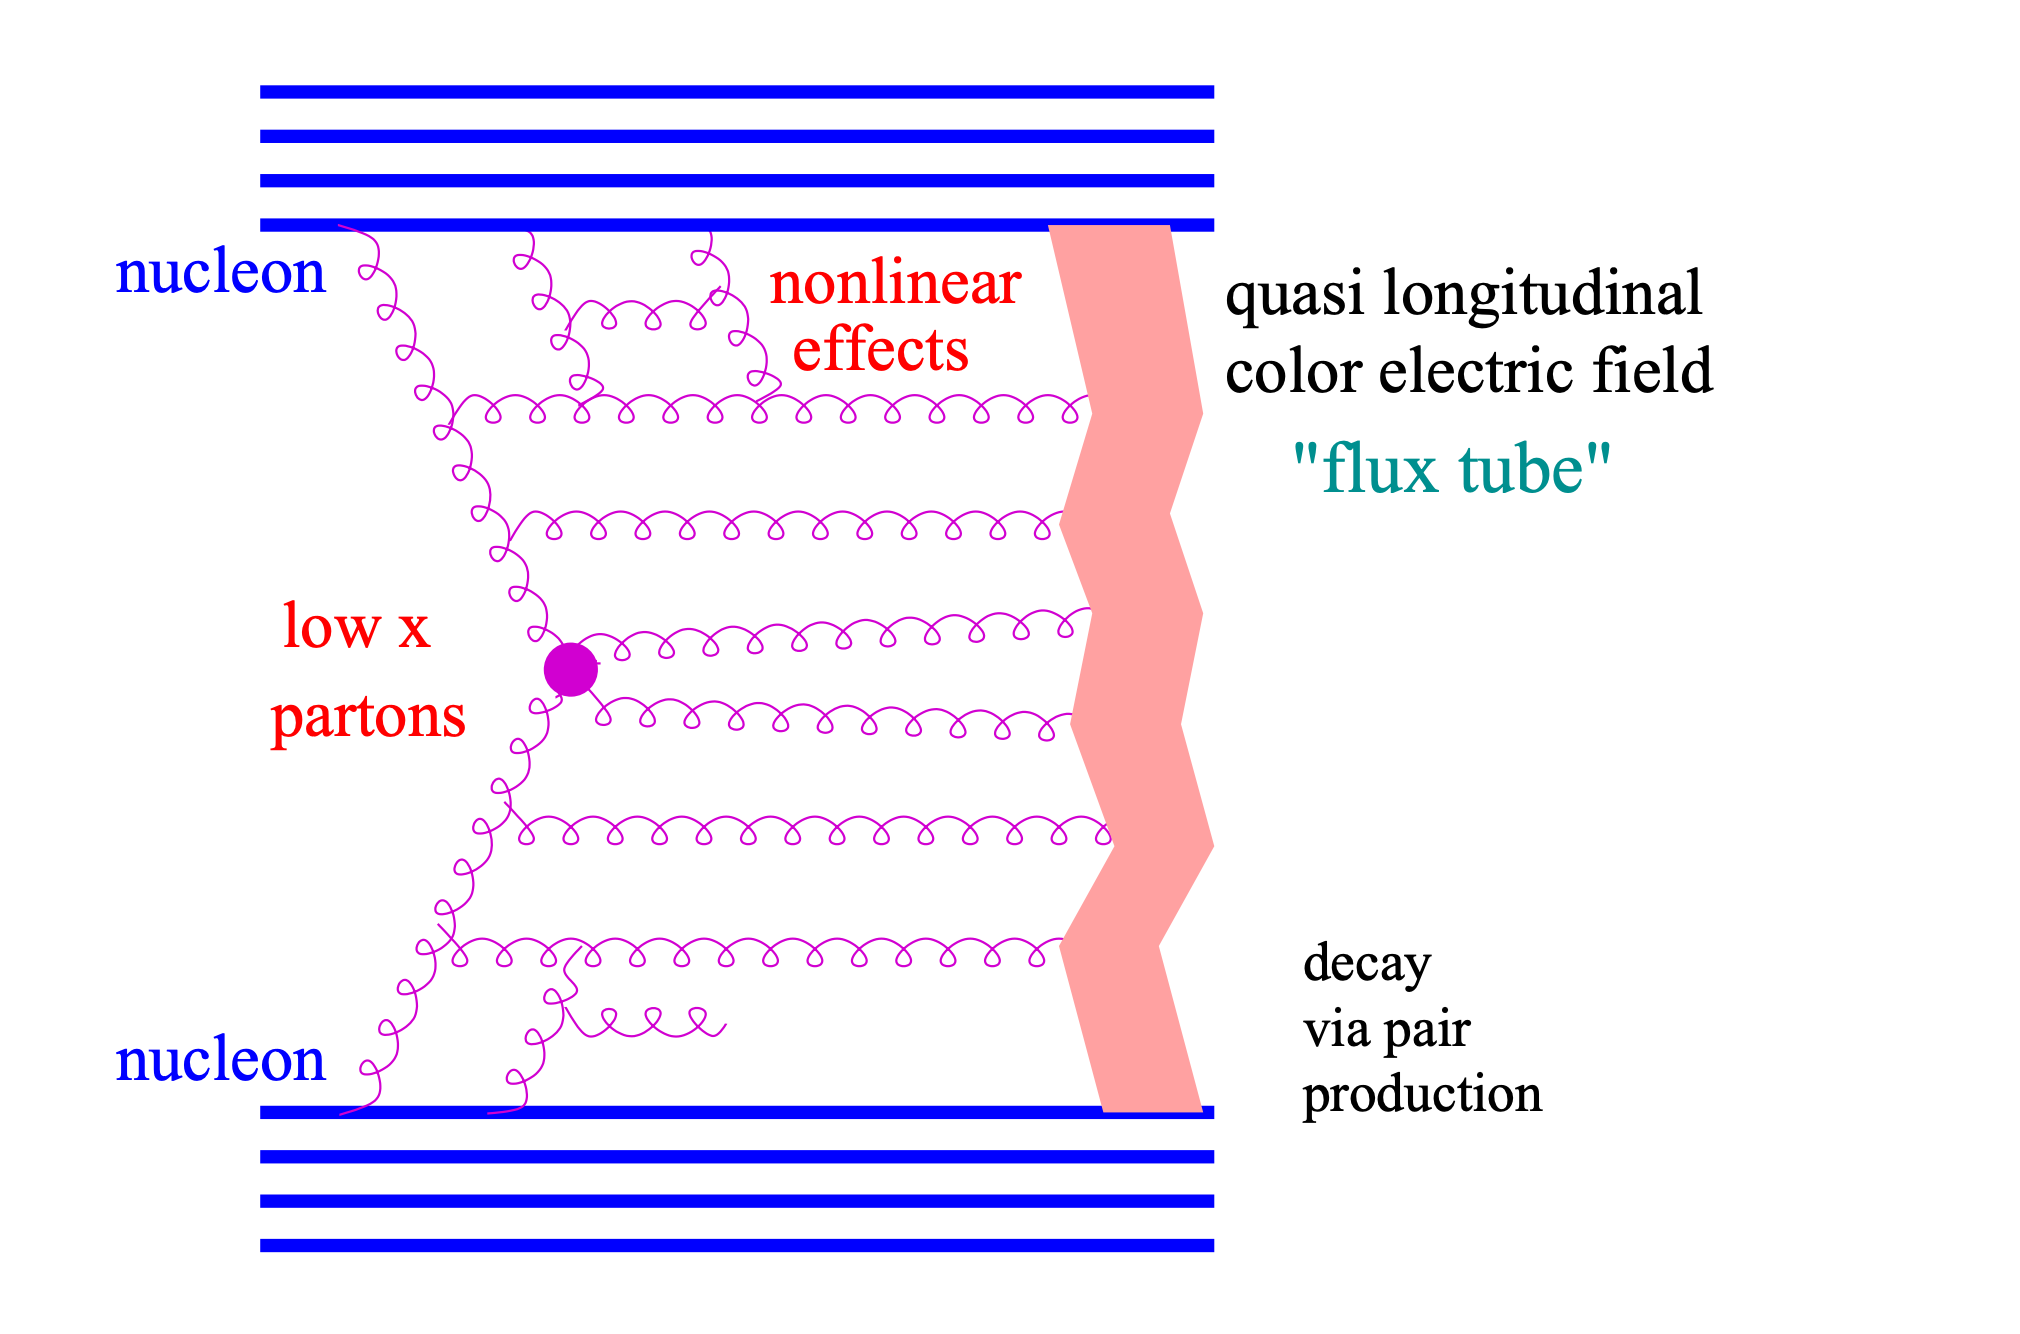
\includegraphics[width=0.7\linewidth]{figures/introduction/epos_interaction.png}
    \caption{A schematic of the elementary interaction in EPOS LHC in which many parton-parton interactions are ocurring simultaneously~\cite{EPOSLHC}.}
    \label{fig:parton_ladder}
\end{figure}

The core is evolved in a hydrodynamic manner, which loses all information about the initial string segments and their interactions. Hadronization in the core is handled by a microcanonical procedure known as Cooper-Frye freeze-out, which is described in detail in~\cite{CooperFrye}. The core is associated with the QGP medium, and dominates particle production at higher multiplicities. The corona, however, corresponds to unmodified Lund string fragmentation, which dominates at large rapidity and in lower multiplicity events. 

\subsection{DPMJET}

Perhaps the most simple\footnote{Still \textit{extremely} complicated from a theoretical perspective, but has the least moving parts.} event generator explored in this thesis is the DPMJET~\cite{DPMJET} model. DPMJET combines the Dual Parton Model (DPM)~\cite{DPM} with the Lund string model~\cite{LundString} to describe proton-proton, proton-nucleus, and nucleus-nucleus collisions across a large range of energies. The DPM describes all of the soft, non-perturbative multi-particle events that occur within a heavy-ion collision using various large $N_c$ and $N_f$ limits of QCD~\cite{DPM}. This is the only model explored in this thesis that does not have an explicit QGP phase, as the collision constituents are always treated independently. Thus, DPMJET serves as a good baseline for vacuum fragmentation, and can be compared with other models (and data) to help quantify the effects of the explicit QGP phase.